%!TeX program = xelatex
\documentclass[aspectratio=169]{beamer}
%\documentclass[aspectratio=169]{beamer}
\usetheme[
outer/progressbar=foot,
outer/numbering=none
]{metropolis} 

\usepackage{amsmath}
\usepackage{pgfplots}
\usepackage{appendixnumberbeamer}
\usepackage[style=authortitle,backend=bibtex]{biblatex}
\addbibresource{references.bib}
\usetikzlibrary{calc} % for manimulation of coordinates
\usepackage{animate}
\makeatletter\def\@anim@pdfmdfivesum#1{#1}\makeatother
\usepackage{tikz}
\usepackage{placeins}
\usepgfplotslibrary{external,fillbetween}
\tikzexternalize
\usetikzlibrary{calc,trees,positioning,arrows,chains,shapes.geometric,%
	decorations.pathreplacing,decorations.pathmorphing,shapes,%
	matrix,shapes.symbols, patterns,shadows.blur}
\tikzset{every picture/.style={/utils/exec={\sffamily}}}
% COLORS FOR GRAPHS

\pgfplotsset{width=\textwidth, height=\textheight*0.33,compat=newest}

\definecolor{train_color_1}{HTML}{8b402a}
\definecolor{train_color_2}{HTML}{e45e2d}
\definecolor{train_color_3}{HTML}{ef9c49}
\definecolor{train_color_4}{HTML}{fdea6f}

\definecolor{test_color_1}{HTML}{192574}
\definecolor{test_color_2}{HTML}{2e62a1}
\definecolor{test_color_3}{HTML}{43a7cb}
\definecolor{test_color_4}{HTML}{9ed5cd}

\pgfplotscreateplotcyclelist{train}{
	semithick,train_color_1\\%
	semithick,train_color_2\\%
	semithick,train_color_3\\%
	semithick,train_color_4\\%
}

\pgfplotscreateplotcyclelist{test}{
	semithick,test_color_1\\%
	semithick,test_color_2\\%
	semithick,test_color_3\\%
	semithick,test_color_4\\%
}

\usepackage{graphicx}
\usetikzlibrary{arrows,positioning}
\usetikzlibrary{calc} % for manimulation of coordinates
\tikzset{
	%Define standard arrow tip
	>=stealth',
	%Define style for boxes
	mylabel/.style={text width=7em, text centered},
	mysmalllabel/.style={text width=7em, text centered},
	punkt/.style={
		rectangle,
		rounded corners,
		draw=black, very thick,
		text width=8em,
		minimum height=2.5em,
		text centered},
	% Define arrow style
	pil/.style={
		->,
		thick,
		shorten <=2pt,
		shorten >=2pt,}
}

\makeatletter
\def\@makefnmark{}
\makeatletter

\tikzset{
	%Define standard arrow tip
	>=stealth',
	%Define style for boxes
	mylabel/.style={text width=7em, text centered},
	mysmalllabel/.style={text width=7em, text centered},
	punkt/.style={
		rectangle,
		rounded corners,
		draw=black, very thick,
		text width=8em,
		minimum height=2.5em,
		text centered},
	punktt/.style={
		rectangle,
		draw=black, thick,
		text width=8em,
		minimum height=2.5em,
		text centered},
	% Define arrow style
	pil/.style={
		->,
		thick,
		shorten <=2pt,
		shorten >=2pt,}
}

\newcommand{\sectiondark}[1]{
	\metroset{background=dark} % change background theme according to manual
	\usebeamercolor[fg]{normal text}
	\section{#1}
	\metroset{background=light} % change background theme according to manual
	\usebeamercolor[fg]{normal text}
}

\usepackage[ruled,vlined]{algorithm2e}
\usepackage{float}
\usepackage{listings}


\lstset{frame=tb,
	language=Python,
	aboveskip=3mm,
	belowskip=3mm,
	showstringspaces=false,
	columns=flexible,
	basicstyle={\small\ttfamily},
	numbers=left,
	numberstyle=\tiny\color{gray},
	keywordstyle=\color{blue},
	commentstyle=\color{dkgreen},
	stringstyle=\color{mauve},
	breaklines=true,
	breakatwhitespace=true,
	tabsize=3,
	inputencoding=latin1
}


\makeatletter
%\setbeamertemplate{title}{
%	\raggedright%
%	\linespread{1.0}%
%	\inserttitle%
%	\par%
%	%\vspace*{0.5em}
%}
\setbeamertemplate{author}{
	\vspace*{2em}
	\begin{minipage}[t]{.2\textwidth}
		{\textbf{Candidate:}}
	\end{minipage}
	\begin{minipage}[t]{.8\textwidth}
	\insertauthor%
	\par%
	\end{minipage}
	\vspace*{0.25em}
}
\setbeamertemplate{date}{
	\hfill
	\insertdate%
	\par%
}
\setbeamertemplate{title page}{	
	\begin{minipage}[b][\paperheight]{\textwidth}
		\vfill%
		\ifx\inserttitle\@empty\else\usebeamertemplate*{title}\fi
		\usebeamertemplate*{title separator}
		\ifx\insertsubtitle\@empty\else\usebeamertemplate*{subtitle}\fi
		\ifx\beamer@shortauthor\@empty\else\usebeamertemplate*{author}\fi
		
		\ifx\insertinstitute\@empty\else\usebeamertemplate*{institute}\fi
		\ifx\inserttitlegraphic\@empty\else\inserttitlegraphic\fi
%		\vspace*{1cm}
		\begin{minipage}[t]{.2\textwidth}
	    	{\small \textbf{Supervisors}:}%
	    	\par%
		\end{minipage}
		\begin{minipage}[t]{.8\textwidth}
			{\small Prof. Pietro Michiardi \hfill EURECOM, France}%
			\par%
			{\small Prof. Elena Baralis \hfill Politecnico di Torino, Italy}%
			\par%
		\end{minipage}
		
		\vfill
		\ifx\insertdate\@empty\else\usebeamertemplate*{date}\fi
		\vfill
		\vspace*{0mm}
	\end{minipage}
}
\makeatother

%\titlegraphic{%
%	\includegraphics[width=.2\textwidth]{example-image-a}\hfill\hfill
%	\includegraphics[width=.2\textwidth]{example-image-b}
%	
%}          % Use metropolis theme
\title{Deep Reinforcement Learning for Autonomous Systems}
\subtitle{\small Designing a control system to exploit model-free deep reinforcement learning algorithms to solve a real-world autonomous driving task of a small robot.}
\date{\today}
\author{Piero Macaluso}
\setbeamercolor{background canvas in title}{parent=palette primary}
\setbeamercolor{progress bar}{use=palette primary}
% \titlegraphic{\hfill
\includegraphics[height=1.5cm]{logo.pdf}}
  
\begin{document}
\metroset{background=dark} % change background theme according to manual
\usebeamercolor[fg]{normal text}
\maketitle
\metroset{background=light} % change background theme according to manual
\usebeamercolor[fg]{normal text}

\begin{frame}
	\begin{center}
		\begin{minipage}{0.4\linewidth}
			\begin{center}
				
\includegraphics[width=1\linewidth]{img/eurecom.png}
				\label{fig:eurecom}
			\end{center}
		\end{minipage}
		\begin{minipage}{0.4\linewidth}
			\begin{center}
				
\includegraphics[width=1\linewidth]{img/polito.png}
				\label{fig:polito}
			\end{center}
		\end{minipage}

		This work of this thesis was developed at EURECOM (Sophia Antipolis, France)\\in collaboration with

		Prof. Pietro Michiardi (EURECOM)\\Prof. Elena Baralis (Politecnico di Torino)
	\end{center}
	\note{
		Good morning,

		Today I am going to present you the work of my thesis project about Deep Reinforcement Learning algorithms applied to Autonomous Systems.
		I developed this thesis during my stay at Eurecom in the south of France under the external supervision of Pietro Michiardi and the internal guidance of prof. Elena Baralis.
	}
\end{frame}

\begin{frame}{Table of contents}
	\setbeamertemplate{section in toc}[sections numbered]
	\tableofcontents[hideallsubsections]
	\note{
		This presentation consists of four main parts:
		\begin{itemize}

			\item 		In the first part, I will outline the crucial concepts underlying autonomous system technology and the reinforcement learning approach. These two research fields are the baseline of this work.
			\item	The second part will be dedicated to the description of the control system we design to make things work together to build up a solid foundation for the reinforcement learning experimentation part. This part represents the first contribution of this thesis.
			\item In the third part, we will discuss the experimental methodology used with a showcase of the results obtained together with a constructive comment.
			\item In the final part, we will analyse what we reached to be able to propose further improvement and research for future work.
		\end{itemize}
	}
\end{frame}

%%%%%%%%%%
% SECTION: Reinforcement Learning Background
%%%%%%%%%%

\sectiondark{Background}

\subsection{State-of-the-art Autonomous Driving Systems}

\begin{frame}{State-of-the-art Autonomous Driving Systems}
	\begin{center}
		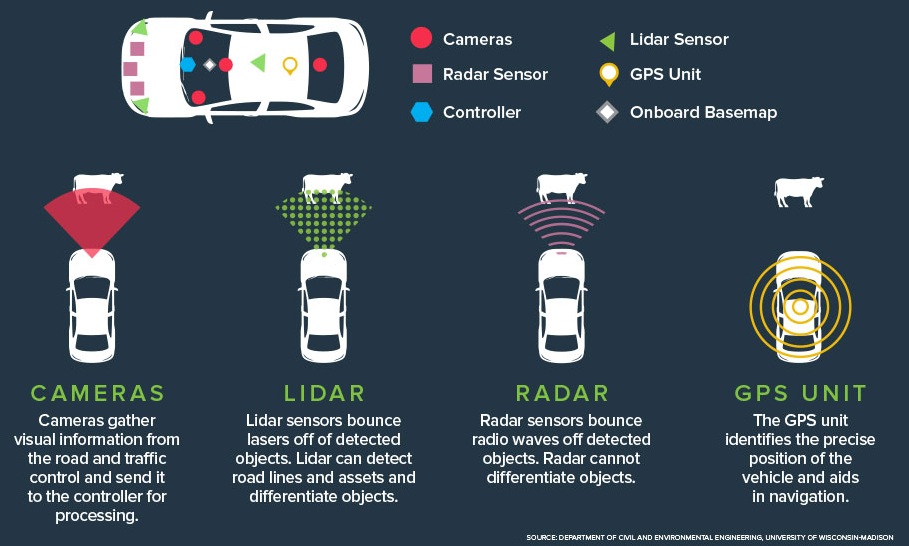
\includegraphics[width=0.8\linewidth]{img/sensors.png}
	\end{center}
	\vspace{-5mm}
	\footcite*{govtech2018aut}



	\note{
		Autonomous systems and self-driving vehicles are attracting much attention from both the research community and industry due to their potential to revolutionise mobility and transport.
		Nowadays, this technology is based on a comprehensive understanding of the surrounding environment. This fact is made possible thanks to the substantial usage of sensors and camera to gather useful information.
		The most crucial sensors used are cameras, LIDAR, Short and Long-range Radar and GPS for coarse localisation.
	}
\end{frame}
%\begin{frame}{State-of-the-art Autonomous Driving Systems}
%	\begin{center}
%		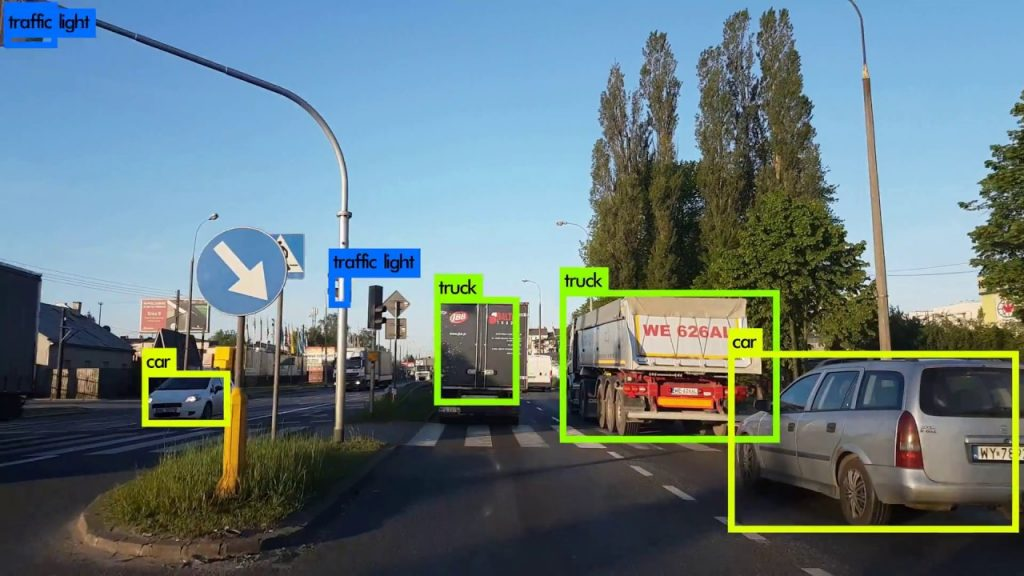
\includegraphics[width=0.7\linewidth]{img/detection.jpg}
%
%
%		\textbf{Deep Learning} and \textbf{Machine Learning} are mainly exploited in\\ \alert{\textbf{object detection}} and \alert{\textbf{recognition}}.
%	\end{center}
%	\note{In this scenario, Deep Learning and Machine Learning are mainly exploited for object detection and recognition, while the implementation of the decision-making component is left to control optimisation algorithms.}
%\end{frame}

\begin{frame}{State-of-the-art Autonomous Driving Systems}
	
	\begin{center}
		\scalebox{0.7}{
			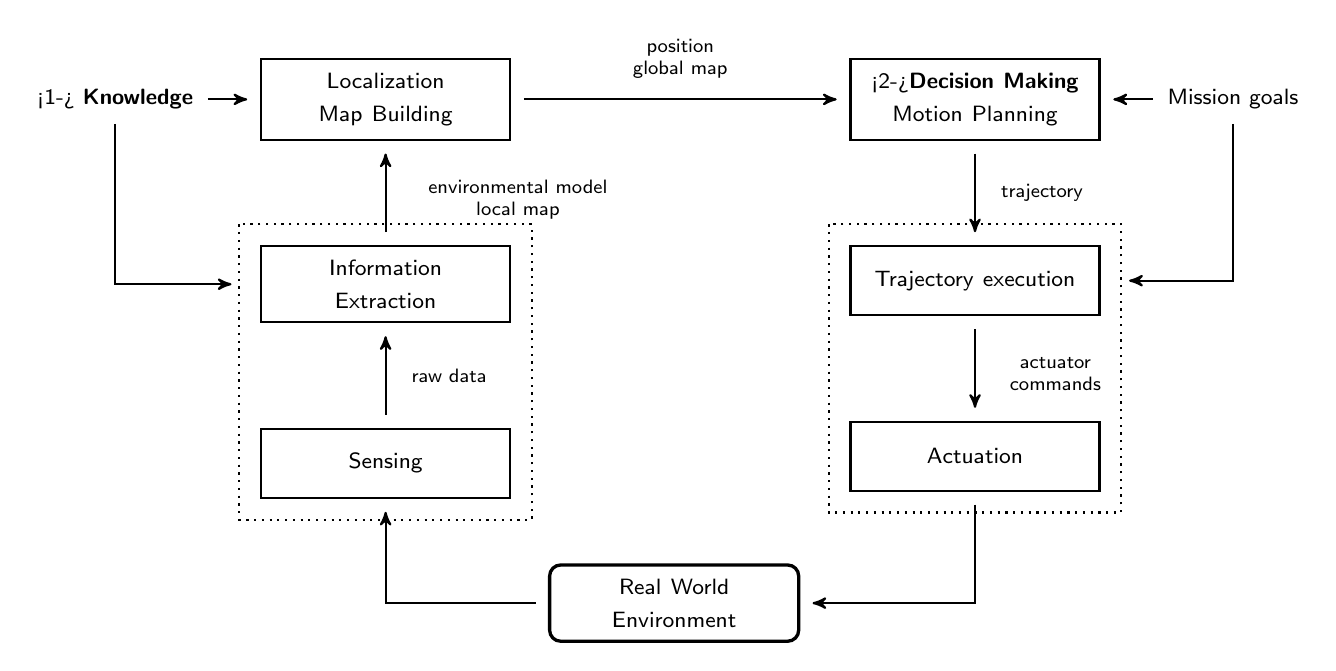
\begin{tikzpicture}
			\node[outer sep=2pt] (knowledge) {\footnotesize \alert<1->{
					\textbf{Knowledge}}};
			\node[punktt,inner sep=5pt,outer sep=5pt,right=0.5cm of knowledge] (localization) {\footnotesize Localization Map Building};
			\node[punktt,inner sep=5pt,outer sep=5pt,below=1cm of localization] (information) {\footnotesize Information Extraction};
			\node[punktt,inner sep=5pt,outer sep=5pt,below=1cm of information] (sensing) {\footnotesize Sensing};
			
			\draw[->, thick](knowledge.east) -- (localization.west);
			\draw[->, thick](sensing.north) -- (information.south) node [midway, right=0.2cm] {\scriptsize raw data};
			\draw[->, thick](information.north) -- (localization.south) node [midway, above right=-0.5cm and 0.2cm] {\scriptsize {\begin{tabular}{c}
					environmental model \\
					local map           \\
					\end{tabular} }};
			\draw[->, thick](knowledge.south) |- ($(information.west) + (-0.2,0)$);
			\draw[black,thick,dotted] ($(information.north west)+(-0.1,0.1)$)  rectangle ($(sensing.south east)+(0.1,-0.1)$);
			
			\node[outer sep=2pt, right=12cm of knowledge] (mission) {\footnotesize Mission goals};
			\node[punktt,inner sep=5pt,outer sep=5pt,left=0.5cm of mission] (decision) {\footnotesize \alert<2->{\textbf{Decision Making}} \\ Motion Planning};
			\node[punktt,inner sep=5pt,outer sep=5pt,below=1cm of decision] (trajectory) {\footnotesize Trajectory execution};
			\node[punktt,inner sep=5pt,outer sep=5pt,below=1cm of trajectory] (actuation) {\footnotesize Actuation};
			
			\node[punkt,inner sep=5pt,outer sep=5pt,below right=0.5cm and 0.15cm of sensing] (environment) {\footnotesize Real World Environment};
			
			\draw[->, thick](mission.west) -- (decision.east);
			\draw[->, thick](decision.south) -- (trajectory.north) node [midway, right=0.2cm] {\scriptsize trajectory};
			\draw[->, thick](trajectory.south) -- (actuation.north) node [midway, above right=-0.5cm and 0.1cm] {\scriptsize {\begin{tabular}{c}
					actuator \\
					commands \\
					\end{tabular} }};
			\draw[->, thick](mission.south) |- ($(trajectory.east) + (+0.2,0)$);
			\draw[black,thick,dotted] ($(trajectory.north west)+(-0.1,0.1)$)  rectangle ($(actuation.south east)+(0.1,-0.1)$);
			
			\draw[->, thick](localization.east) -- (decision.west) node [midway, above=0.1cm] {\scriptsize {\begin{tabular}{c}
					position   \\
					global map \\
					\end{tabular} }};
			
			\draw[->, thick](actuation.south) |- (environment.east);
			\draw[->, thick](environment.west) -| (sensing.south);
			
			\end{tikzpicture}}
	\end{center}
	\vspace{-7mm}
	\footcite*{pavone2019veicoli}
	
	\note<1>{This schema outlines the crucial components of the modern autonomous driving car technology together with the interactions among them.
		\begin{itemize}
			\item At the bottom, we have the surrounding environment.
			\item In the left section, we have a stack of components from the raw data to feature extraction.
			\item The right section is the decision-making part, where the algorithm decided what action to make.
		\end{itemize}
		
		Nowadays, we find the application of ML and DL only in the left part to extract features that a control optimisation algorithm will exploit to select what to do deterministically. }
	\note<2>{The idea underlying this project is trying to implement artificial intelligence inside this decision-making part.}
	
\end{frame}


\begin{frame}{Reinforcement Learning}
	Problems involving an \textbf{agent}
	interacting with an \textbf{environment}
	, which provides numeric \textbf{reward signals}.

	\onslide<2->{\alert{\textbf{Goal}}: Learn how to take actions in order to maximize a reward function.}

	\begin{center}
		\scalebox{0.9}{
			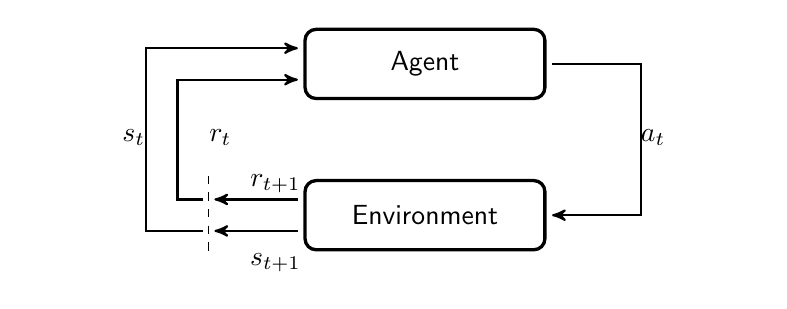
\begin{tikzpicture}
				% node Agent
				\node[punkt] (agent) {Agent};
				% node Environment
				\node[punkt, below=1cm of agent] (env) {Environment};
				% node a_t
				\node[mylabel, below right=0.25cm and 0cm of agent] (action) {$a_t$};
				% node s_t
				\node[mylabel, below left=0.25cm and 0.8cm of agent] (state) {$s_t$};
				% node r_t
				\node[mylabel, below left=0.25cm and -0.3cm of agent] (reward) {$r_t$};
				% node s_t+1
				\node[mylabel, above left=-1.3cm and -1cm of env] (state) {$s_{t+1}$};
				% node r_t+1
				\node[mylabel,above left=-.3cm and -1cm of env] (reward1) {$r_{t+1}$};
				\draw[pil]   (agent.east) -- ($(agent.east) + (1.2cm,0cm)$)  |-  (env.east);
				\draw[pil]   ($(env.west) + (0,-0.2cm)$) -- ($(env.west) + (-1.2cm,-0.2cm)$);
				\draw[pil]   ($(env.west) + (-1.2cm,-0.2cm)$) -- ($(env.west) + (-2cm,-0.2cm)$) |-($(agent.west) + (0,0.2cm)$);
				\draw[pil]   ($(env.west) + (0,+0.2cm)$) -- ($(env.west) + (-1.2cm,+0.2cm)$);
				\draw[pil]   ($(env.west) + (-1.2cm,+0.2cm)$) -- ($(env.west) + (-1.6cm,+0.2cm)$) |-($(agent.west) + (0,-0.2cm)$);
				\draw[dashed]  ($(env.west) - (1.2cm,-0.5cm)$) -- ($(env.west) - (1.2cm,0.5cm)$);
			\end{tikzpicture}
			\label{looprl}
			\footcite*{sutton2018reinforcement}
		}
	\end{center}

	\note{
		Reinforcement Learning is a paradigm of machine learning that formalises and tries to solve decision-making tasks. In this formalisation, we can find:
		\begin{itemize}
			\item The agent - the brain, the entity that makes decisions.
			\item The environment: it is everything external to the agent.
			\item The actions, the mean by which agent can interact and influence the environment.
		\end{itemize}
	}
\end{frame}

\begin{frame}{From Data to Value}
	\onslide<1->{}	% \onslide<2->{}
	\begin{center}
		%		\includegraphics<1>[width=\linewidth]{img/reinforcement-learning-1.png}
		\includegraphics<1>[width=\linewidth]{img/reinforcement-learning-2.png}
	\end{center}
	\footcite*{chara2018wild}
\end{frame}

\begin{frame}{Algorithms implemented}
	\begin{columns}
		\begin{column}{0.5\linewidth}
			\begin{itemize} % [<+- | alert@+>]
				\item \textbf{Model-Free}
				\item \textbf{Off-Policy} with \textbf{Experience Replay Memory} of $(s_t, a_t, r_t, s_{t+1}, d_t)$ tuples
				\item \textbf{Continuous} Action space
				\item \textbf{Actor-Critic} approach
			\end{itemize}
		\end{column}
		\begin{column}{0.5\linewidth}
			\centering
			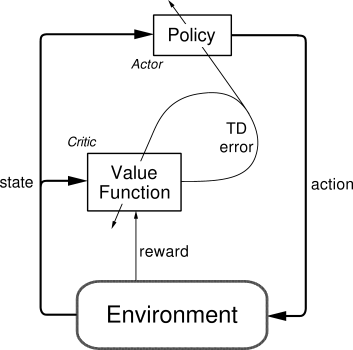
\includegraphics[width=0.8\linewidth]{img/actor_critic.png}
		\end{column}
	\end{columns}
	\footcite*{sutton2018reinforcement}

\end{frame}

\begin{frame}{Deep Deterministic Policy Gradient (DDPG)}
	\centering
	\onslide<5>{}
	DDPG learns a Q-function and a policy. It uses off-policy data and the Bellman equation to learn the Q-function, and uses the Q-function to learn the policy.
	\begin{itemize}[<+- | alert@+>]
		\item \textbf{Policy}: Deterministic
		\item \textbf{Exploration}: \begin{itemize}
			      \item \textbf{Ornstein–Uhlenbeck} process noise
			      \item Noise regulation with \textbf{$\epsilon$-decay function}
		      \end{itemize}
	\end{itemize}
	\onslide<5->{\textbf{\alert{\underline{Needs accurate hyper-parameters fine-tuning}}}}
	\footcite*{lillicrap2015continuous}
\end{frame}

\begin{frame}{Soft Actor-Critic (SAC)}
	\onslide<5>{}
	SAC learns a policy and two Q-functions. It exploits \textbf{entropy regularization}. \note{The policy is trained to maximize a trade-off between expected return and \textbf{entropy}. Entropy is a measure of randomness in the policy.}
	\centering
	\begin{itemize}[<+- | alert@+>]
		\item \textbf{Policy}: Stochastic
		\item \textbf{Exploration}: \begin{itemize}[<+- | alert@+>]
			      \item \textbf{Temperature} Parameter
			      \item \textbf{Auto-tuning}
		      \end{itemize}
	\end{itemize}
	\onslide<5->{\textbf{\alert{\underline{Suitable for Real-World Experiments}}}}
	\footcite*{haarnoja2018alg}
\end{frame}

\begin{frame}{Main Goals}
	\begin{columns}
		\begin{column}{0.4\linewidth}
			\centering
			
\includegraphics[width=0.6\linewidth]{img/goal.png}
		\end{column}
		\begin{column}{0.6\linewidth}
			\begin{enumerate}%[<+- | alert@+>]
				\item{Implementation of Reinforcement Learning algorithms}
				\begin{itemize}
					\item{Preliminary experiments on a simplified environment}
				\end{itemize}
				\item{Building a \textbf{control system} binding every technology used.}
				\begin{itemize}
					\item{Formalise the problem as MDP}
				\end{itemize}
				\item \textbf{Real World} Reinforcement Learning experiments analysis.
				\begin{itemize}
					\item\textbf{No model} of the environment.
					\item\textbf{No preliminary simulation} to tune hyper-parameters
				\end{itemize}
			\end{enumerate}
		\end{column}
	\end{columns}
\end{frame}



\sectiondark{Design of the control system}

\begin{frame}{Anki Cozmo - Not just a toy robot}
	\begin{columns}
		\begin{column}{0.5\linewidth}
			\begin{center}
				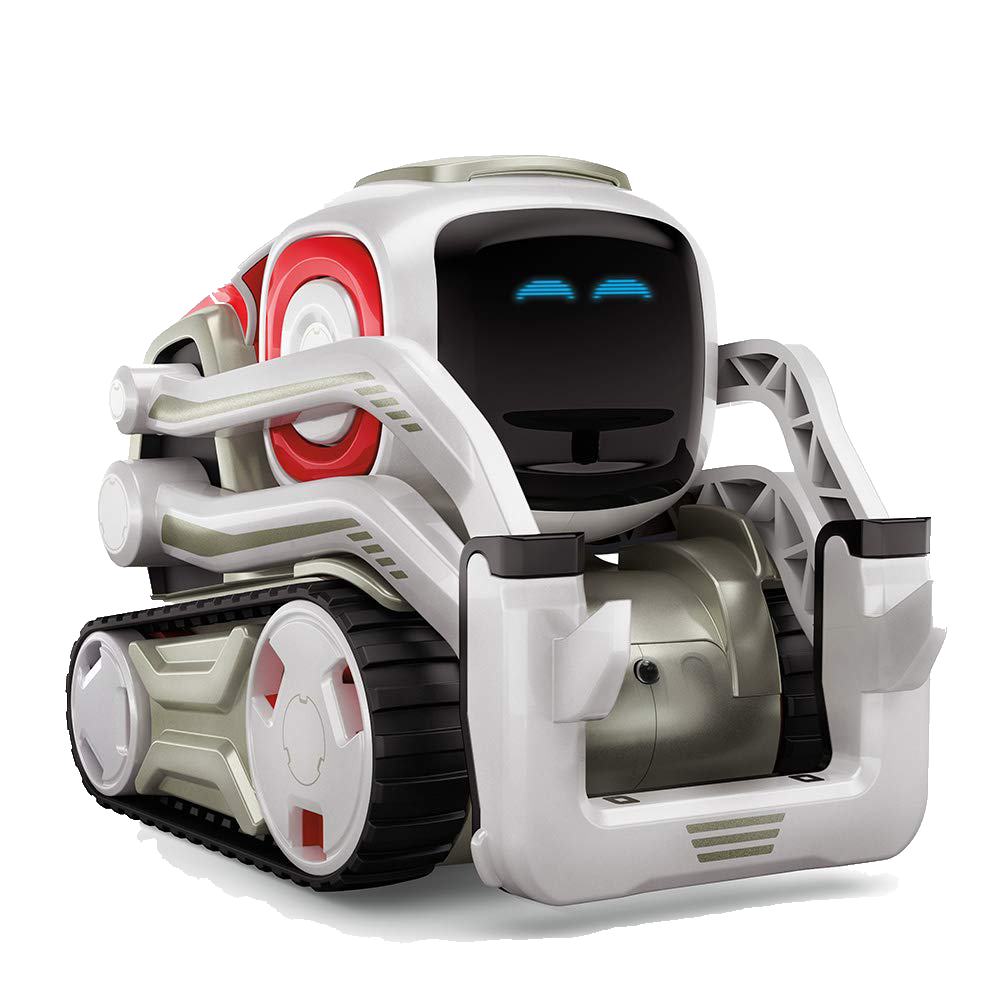
\includegraphics[height=0.5\linewidth]{img/cozmo.png}
				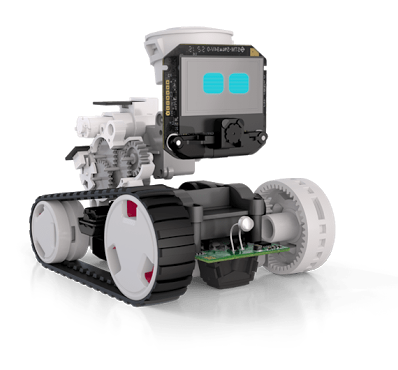
\includegraphics[height=0.5\linewidth]{img/cozmo_inside.png}
			\end{center}
		\end{column}
		\begin{column}{0.5\linewidth}
			\textbf<1->{Why Anki Cozmo?}
			\begin{itemize}%[<+- | alert@+>]
				\item{Small and portable}
				\item{30fps VGA Camera}
				\item{Powerful mechanics}
				\item{\textbf{Python SDK and interfaces}}
			\end{itemize}
		\end{column}
	\end{columns}
\end{frame}

\begin{frame}{Track Design}
	\centering
	\begin{columns}
		\begin{column}{0.5\linewidth}
			\begin{center}
				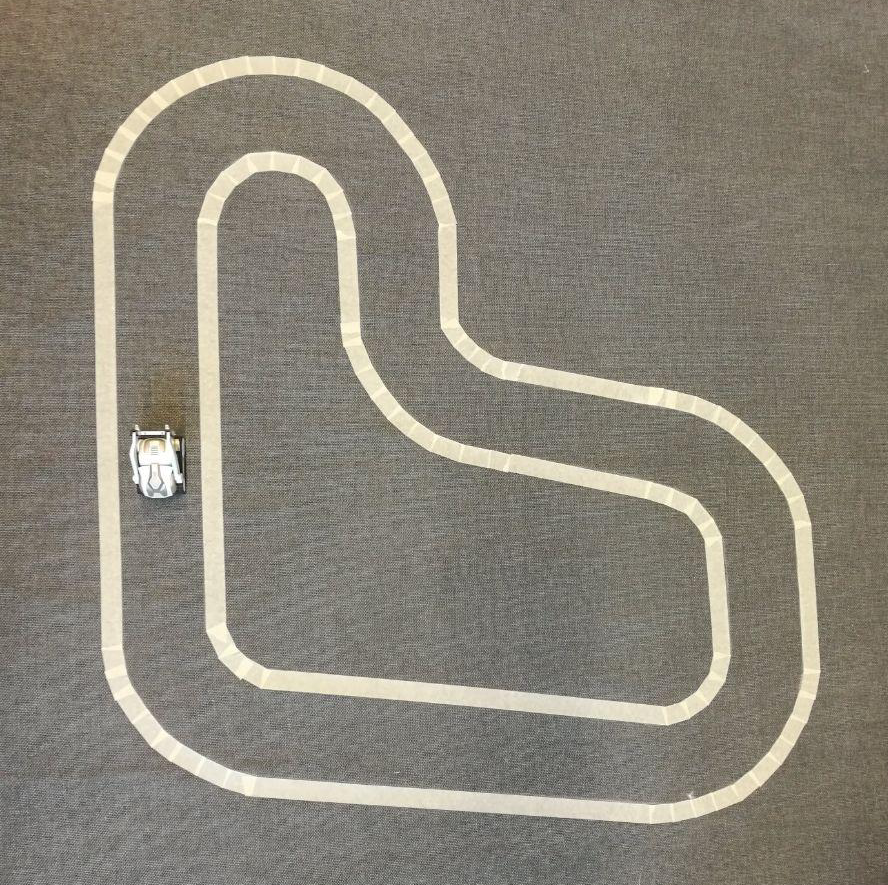
\includegraphics[height=0.6\textheight]{img/track.png}
			\end{center}
		\end{column}
		\begin{column}{0.5\linewidth}
			\textbf<1->{Features:}
			\begin{itemize}%[<+- | alert@+>]
				\item{Low-reflections}
				\item{Scaled Reality}
				\item{Reproducible}
			\end{itemize}
		\end{column}
	\end{columns}
\end{frame}

\begin{frame}{MDP Formalisation - Observation}
	\begin{columns}
		\begin{column}{0.5\linewidth}
			\centering
			\only<1>{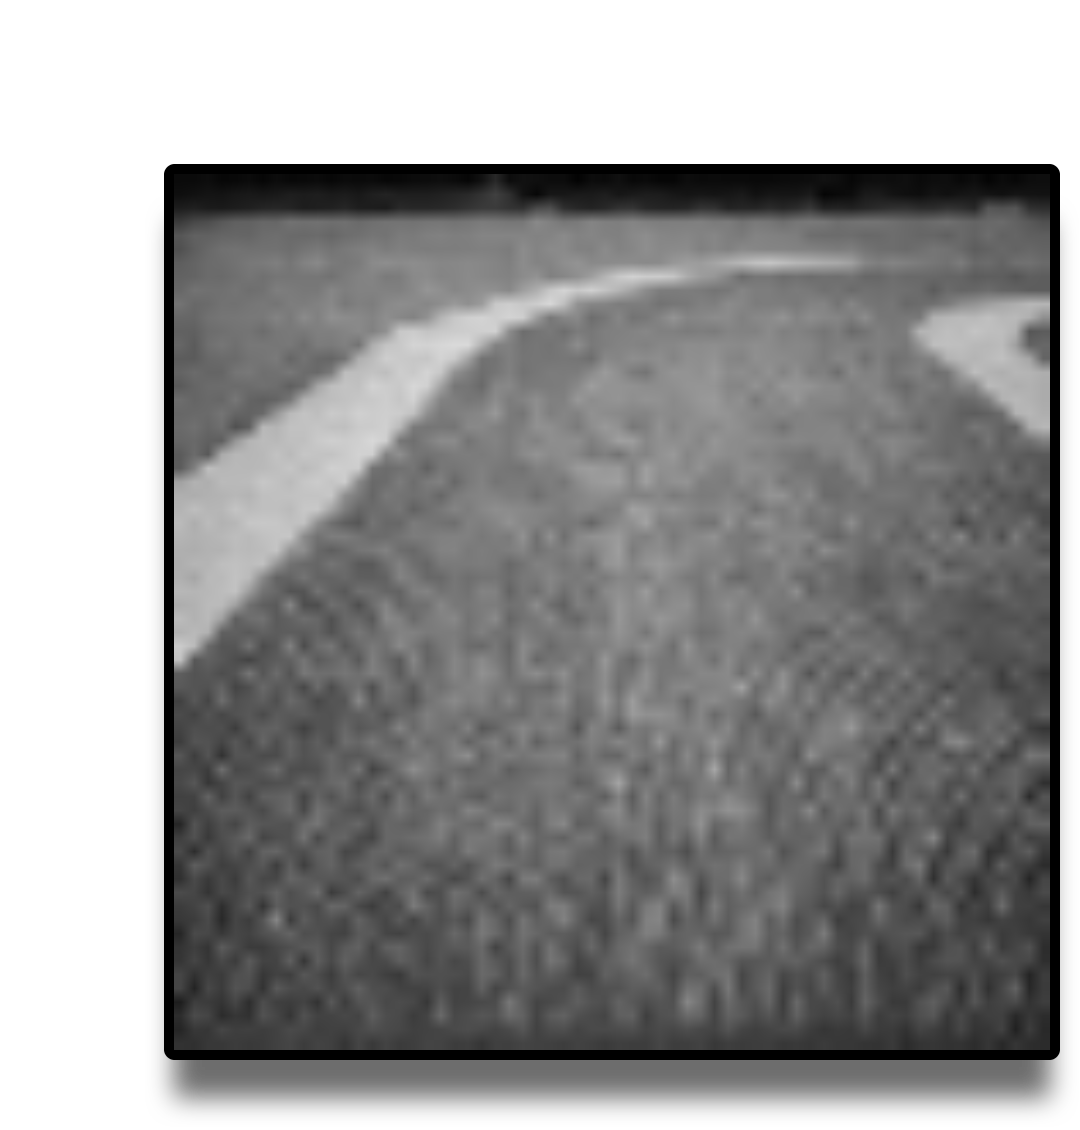
\includegraphics[height=0.6\textheight]{img/obs1.png}}

			\only<2>{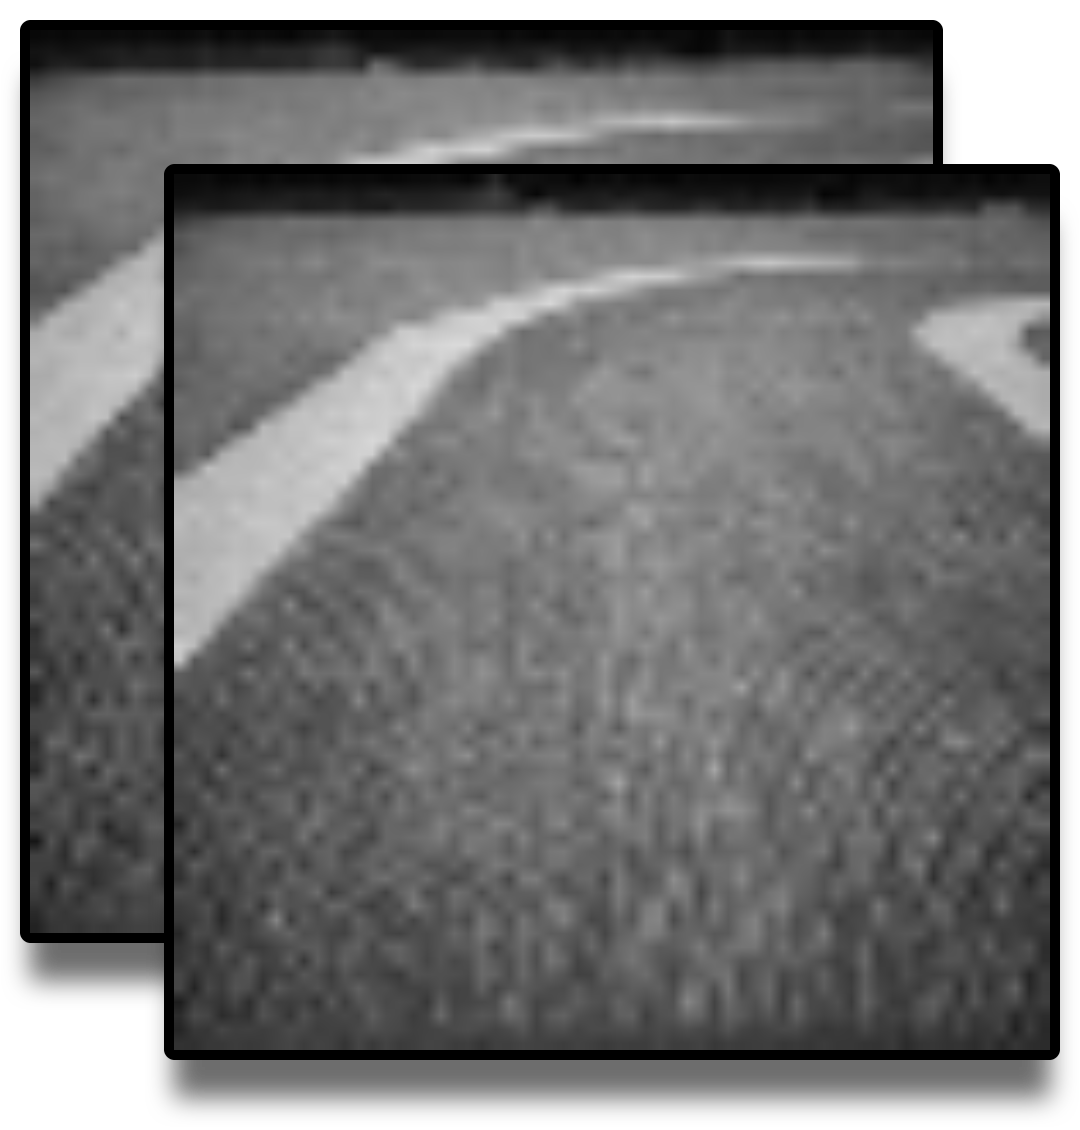
\includegraphics[height=0.6\textheight]{img/obs2.png}}
		\end{column}
		\begin{column}{0.5\linewidth}
			\textbf{Configuration:}
			\begin{itemize}%[<+- | alert@+>]
				\item\textbf{Gray-scale image}
				\item\textbf{Frame Rate}: $\sim 15fps$
				\item\textbf{Raw image size}: 64$\times$64 pixels
				\item<2>\textbf{Stack size}: 2
			\end{itemize}
		\end{column}
	\end{columns}
\end{frame}

\begin{frame}{MDP Formalisation - Actions}
	
\includegraphics[width=1\textwidth]{img/array.png}
	\begin{equation*}
		s_t \in \{x \in \mathbb{R} \;|\; 0 \le x \le 1\} \;\;\;\;\;\;
		w_t \in \{x \in \mathbb{R} \;|\; -1 \le x \le 1\}
	\end{equation*}
	\onslide<2->{
		\begin{align*}
			\text{\textbf{Maximum forward speed}} & \rightarrow s_{\text{forward\_max}} = 150\text{mm/s} \\
			\text{\textbf{Maximum turning speed}} & \rightarrow s_{\text{turning\_max}} = 100\text{mm/s}
		\end{align*}
	}
	\onslide<3->{
		\begin{align*}
			\text{\textbf{Left tread speed}}  & \leftarrow s_t \cdot s_{\text{forward\_max}} + w_t \cdot s_{\text{turning\_max}} \\
			\text{\textbf{Right tread speed}} & \leftarrow s_t \cdot s_{\text{forward\_max}} - w_t \cdot s_{\text{turning\_max}}
		\end{align*}
	}

\end{frame}


\begin{frame}{MDP Formalisation - Reward}
	\begin{columns}
		\begin{column}{0.4\linewidth}
			\centering
			
\includegraphics[width=0.8\linewidth]{img/reward.png}
		\end{column}
		\begin{column}{0.6\linewidth}
			\centering
			\textbf{Distance Covered}

			\textbf{Fixed timing between actions}: $T_t$ [s] $\leftarrow \frac{1}{15 \;\text{fps}}$

			\textbf{Desired Speed}: $s_t$ [mm/s]

			\onslide<2->{{\Large
						\begin{equation*}\boldsymbol{
								R_t = s_t \cdot T_t}
						\end{equation*}}}
			\vspace{-5mm}
			\onslide<2->{
				\begin{equation*}
					\text{if}\; t\; \text{is terminal} \rightarrow R_t = 0
				\end{equation*}}
		\end{column}
	\end{columns}
\end{frame}

\begin{frame}{Outline of the control system}
	\centering

	\only<1>{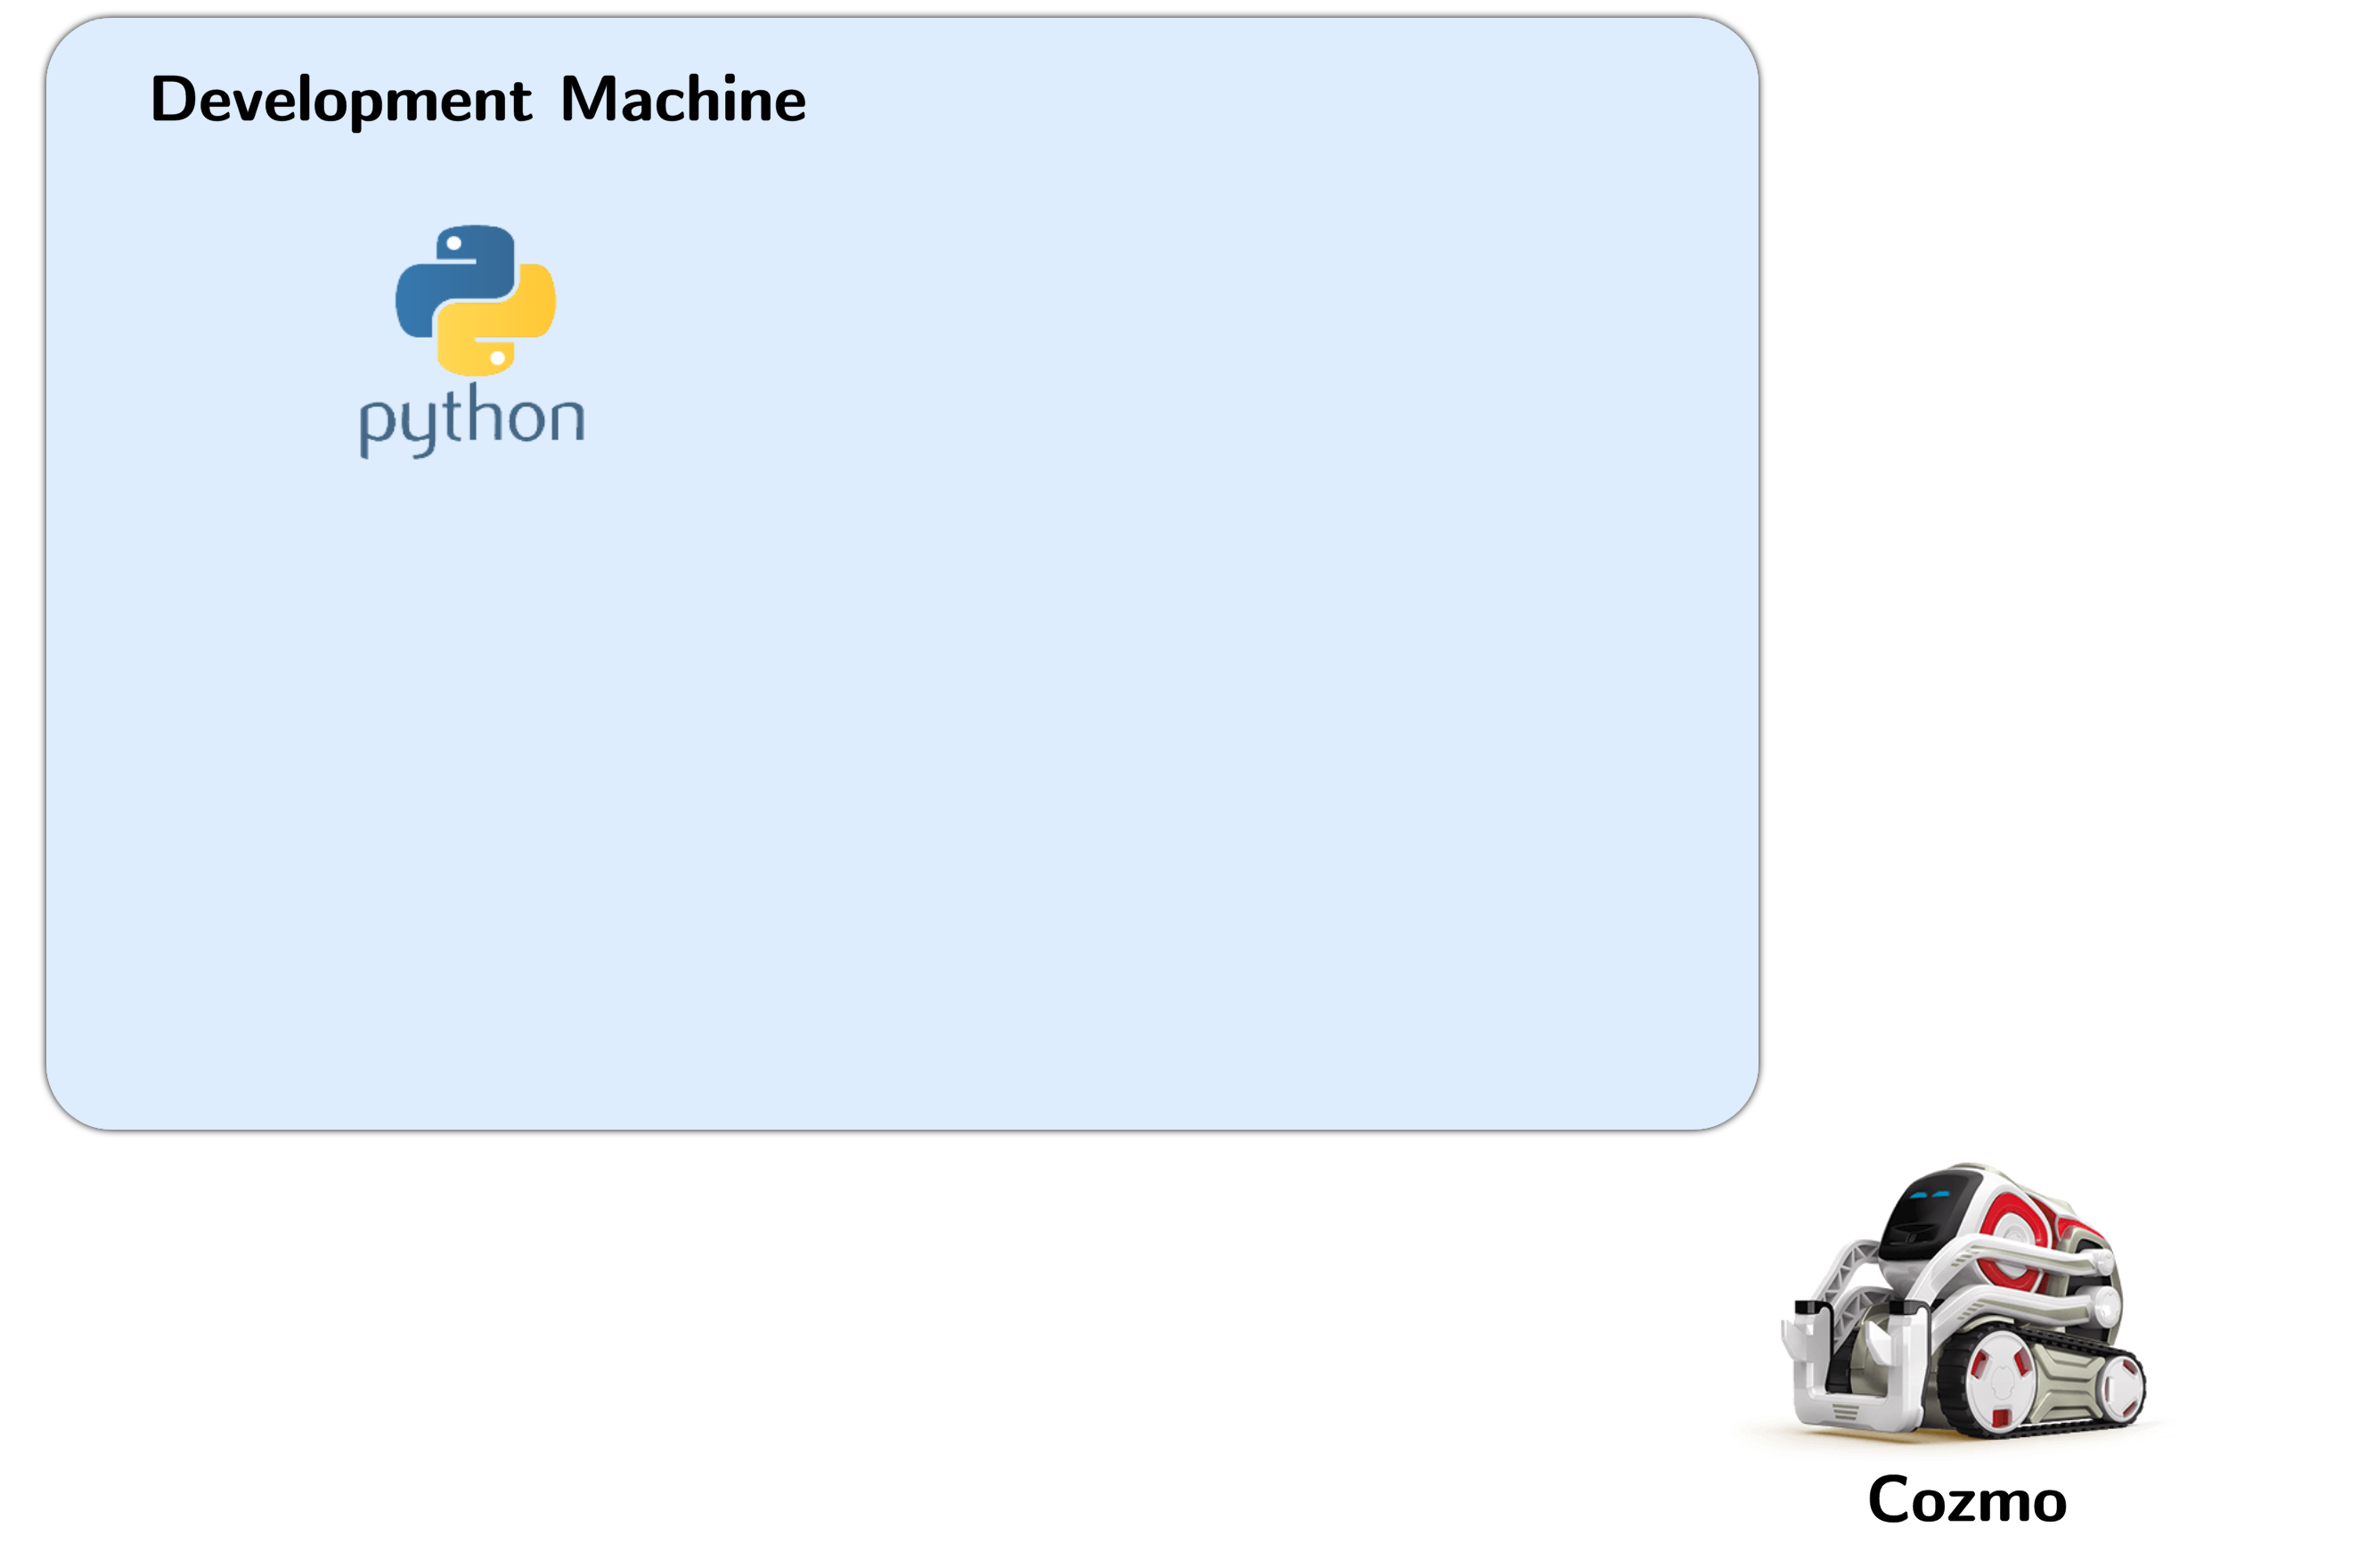
\includegraphics[height=0.9\textheight]{img/cozmosys0.png}}

	\only<2>{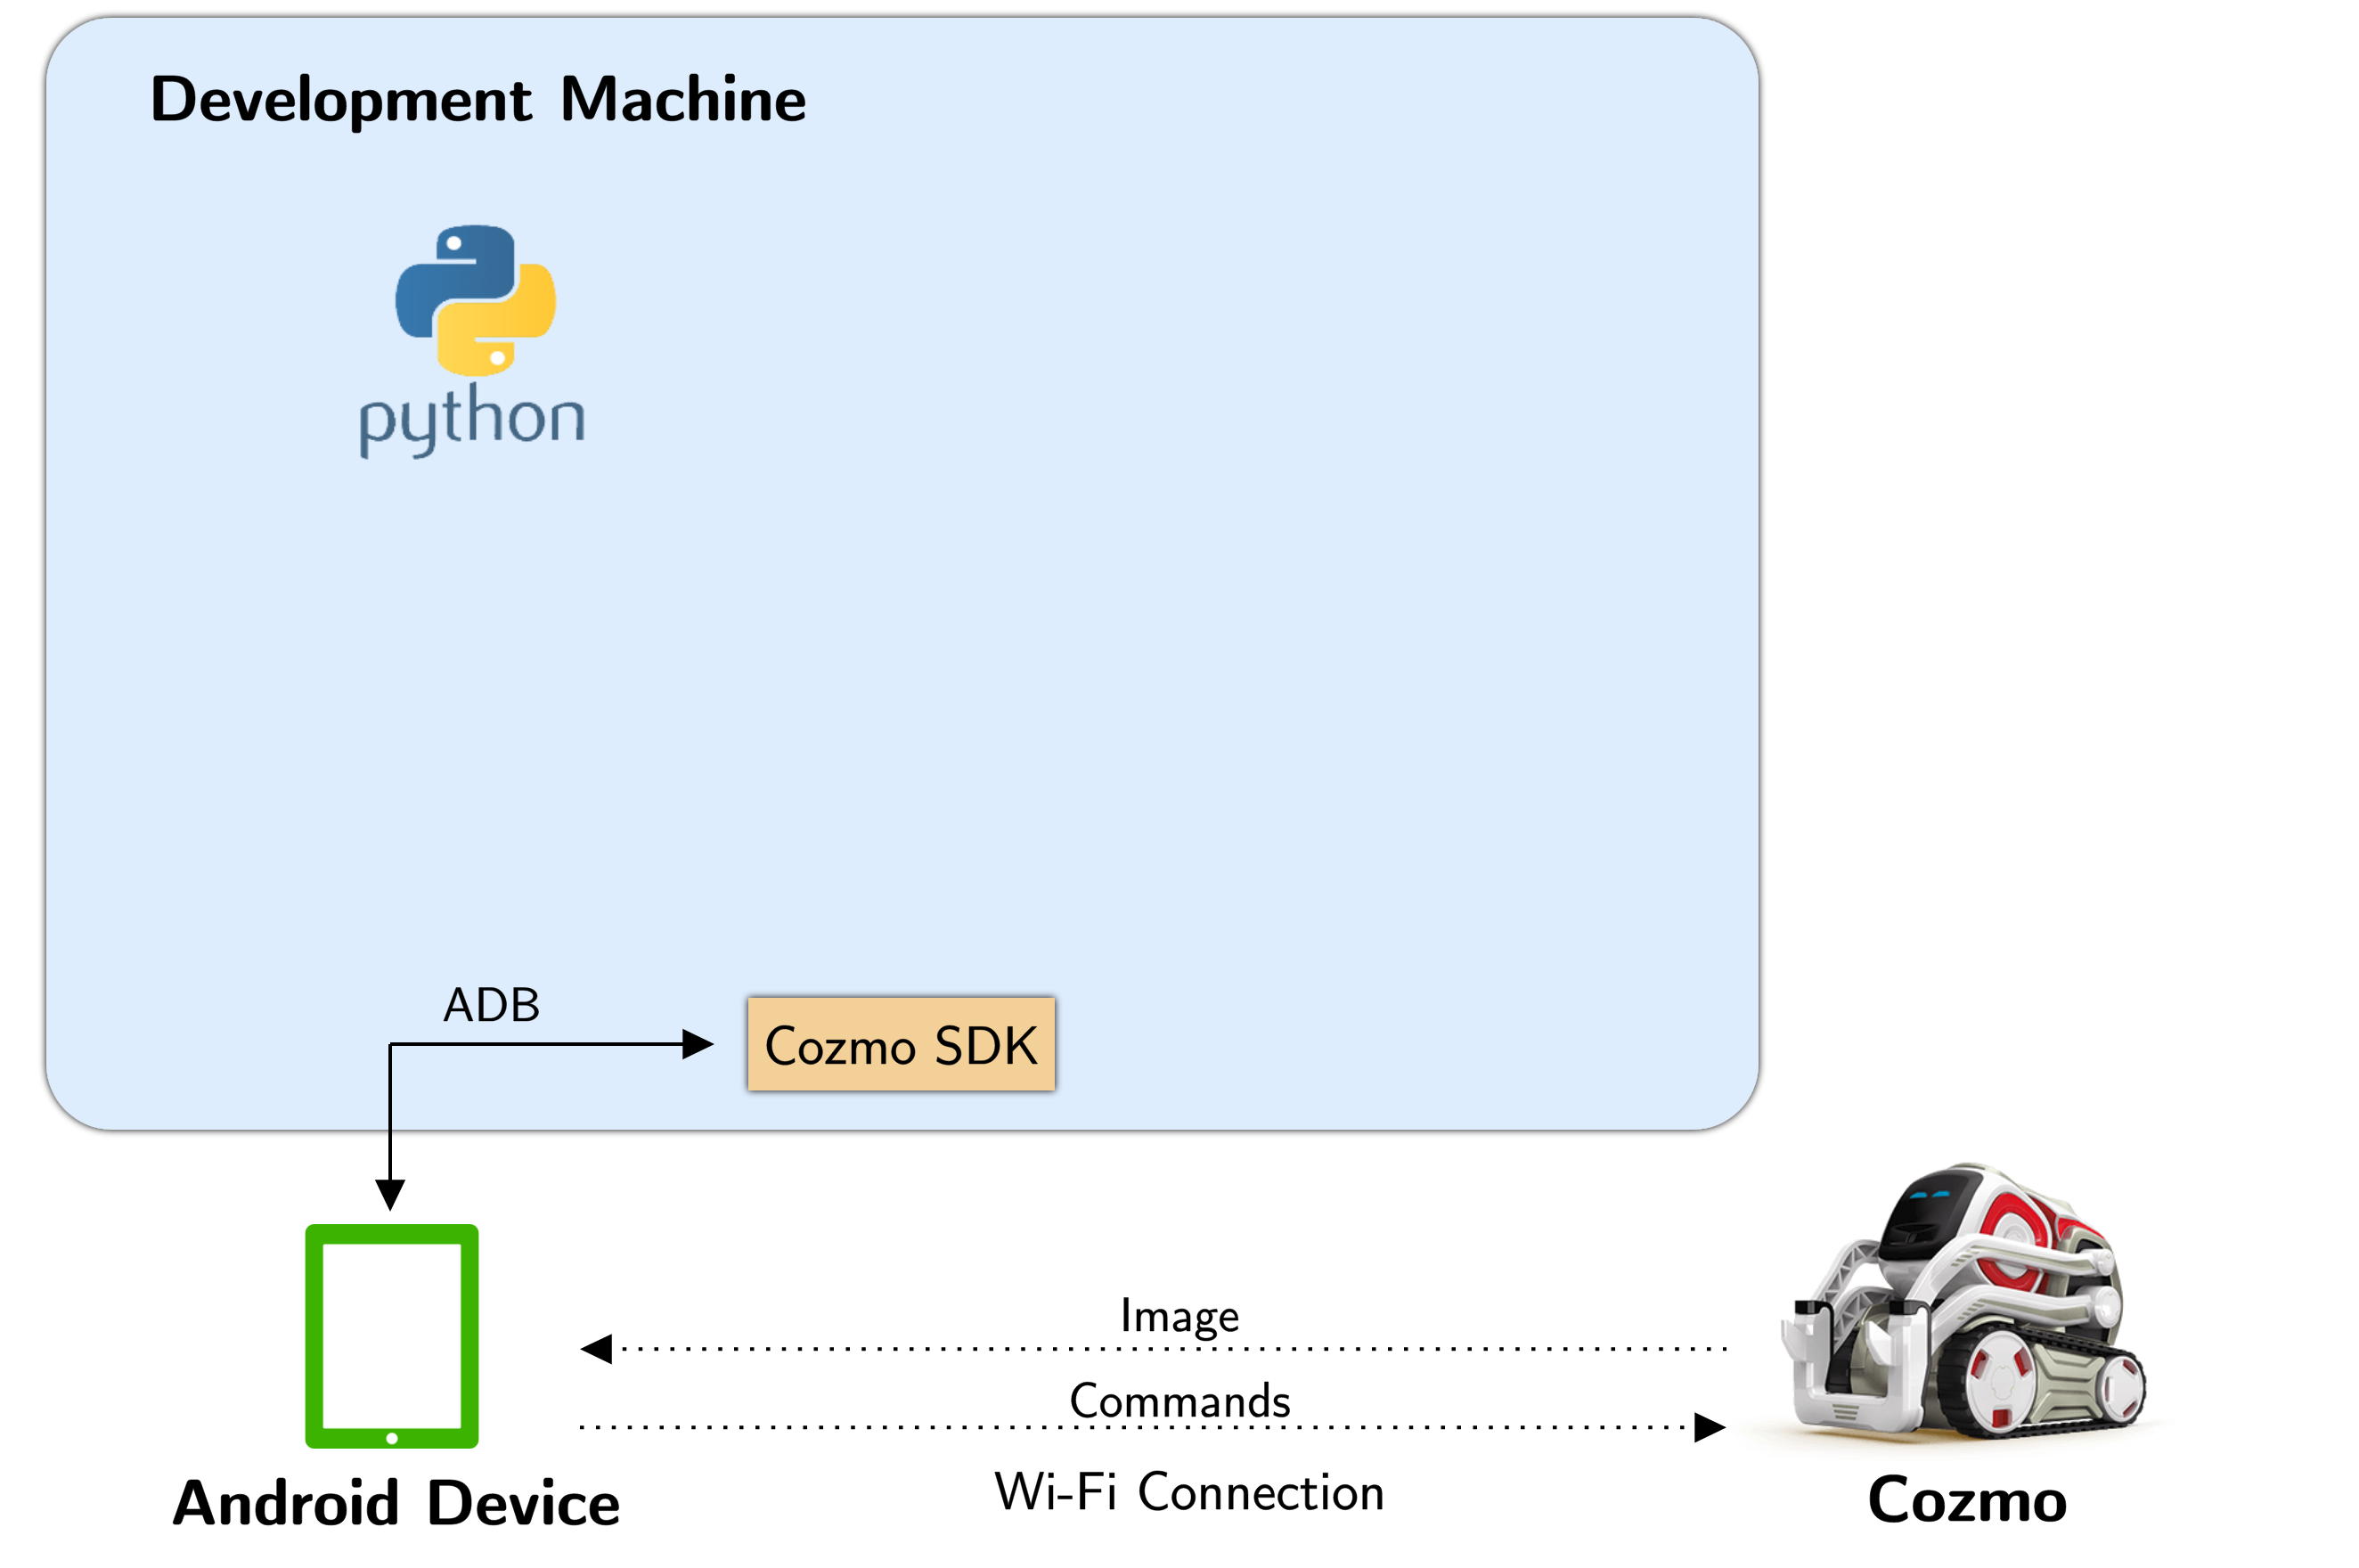
\includegraphics[height=0.9\textheight]{img/cozmosys1.png}}

	\only<3>{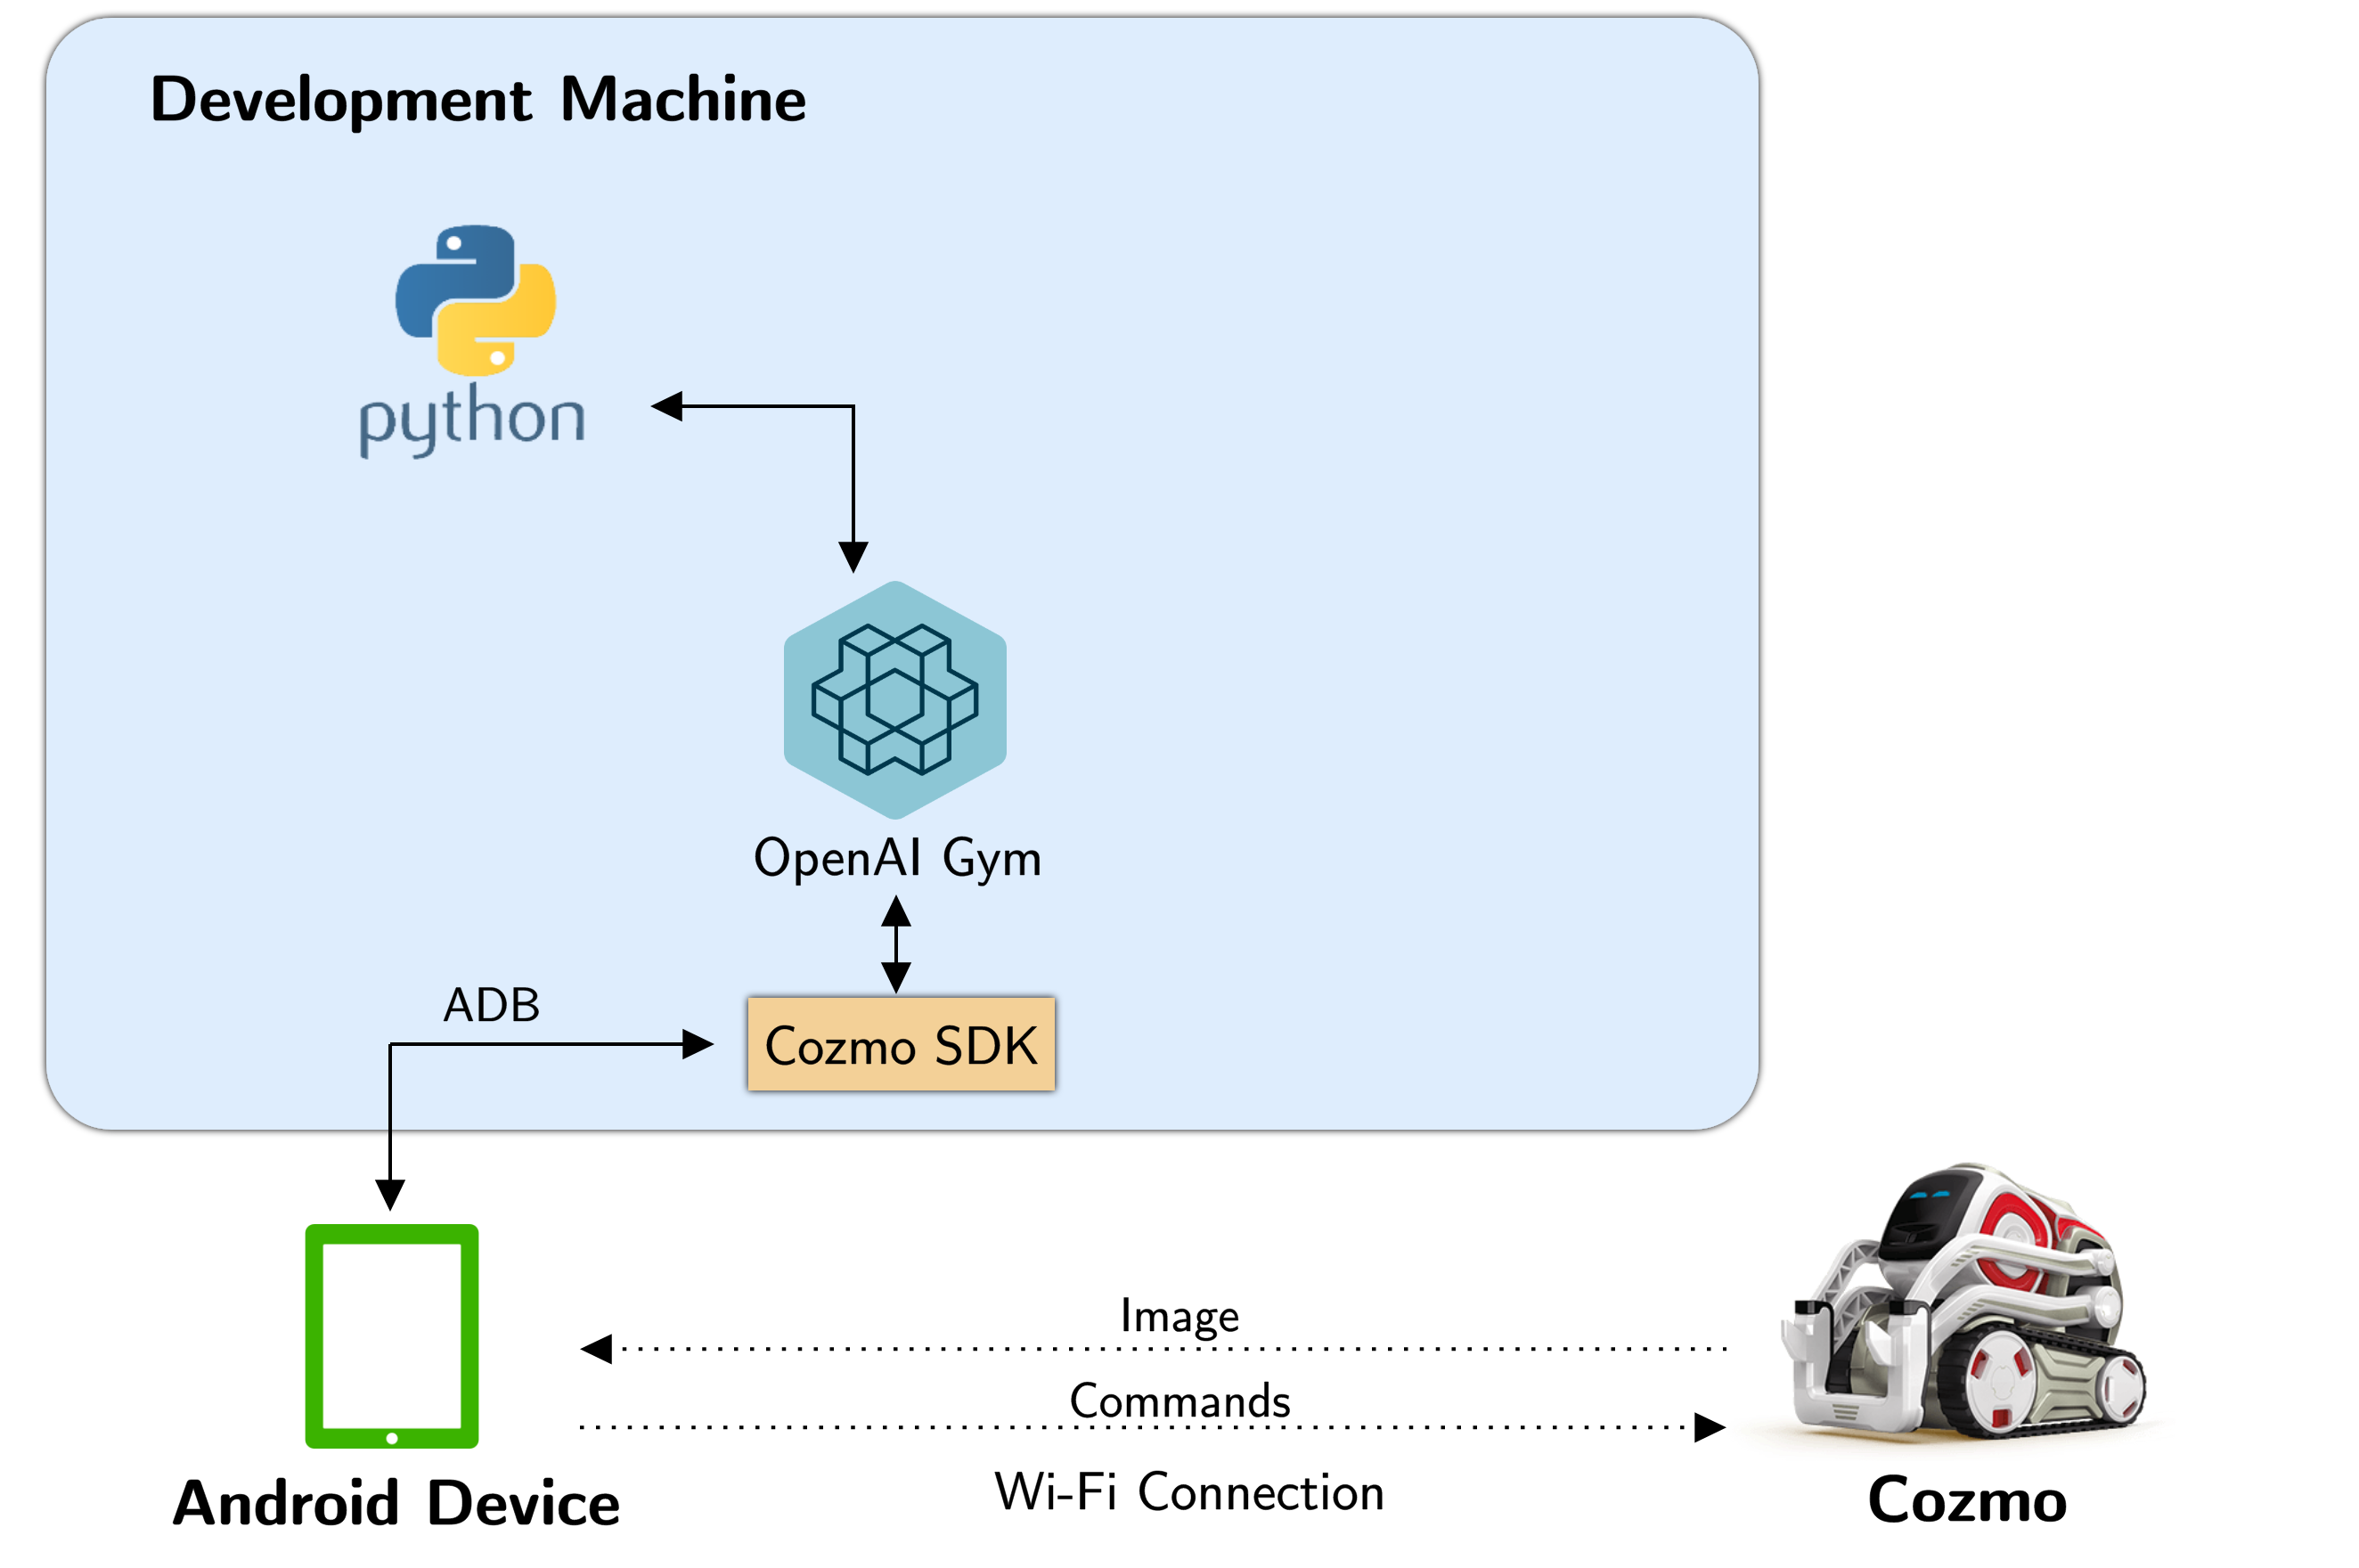
\includegraphics[height=0.9\textheight]{img/cozmosys2.png}}

	\only<4>{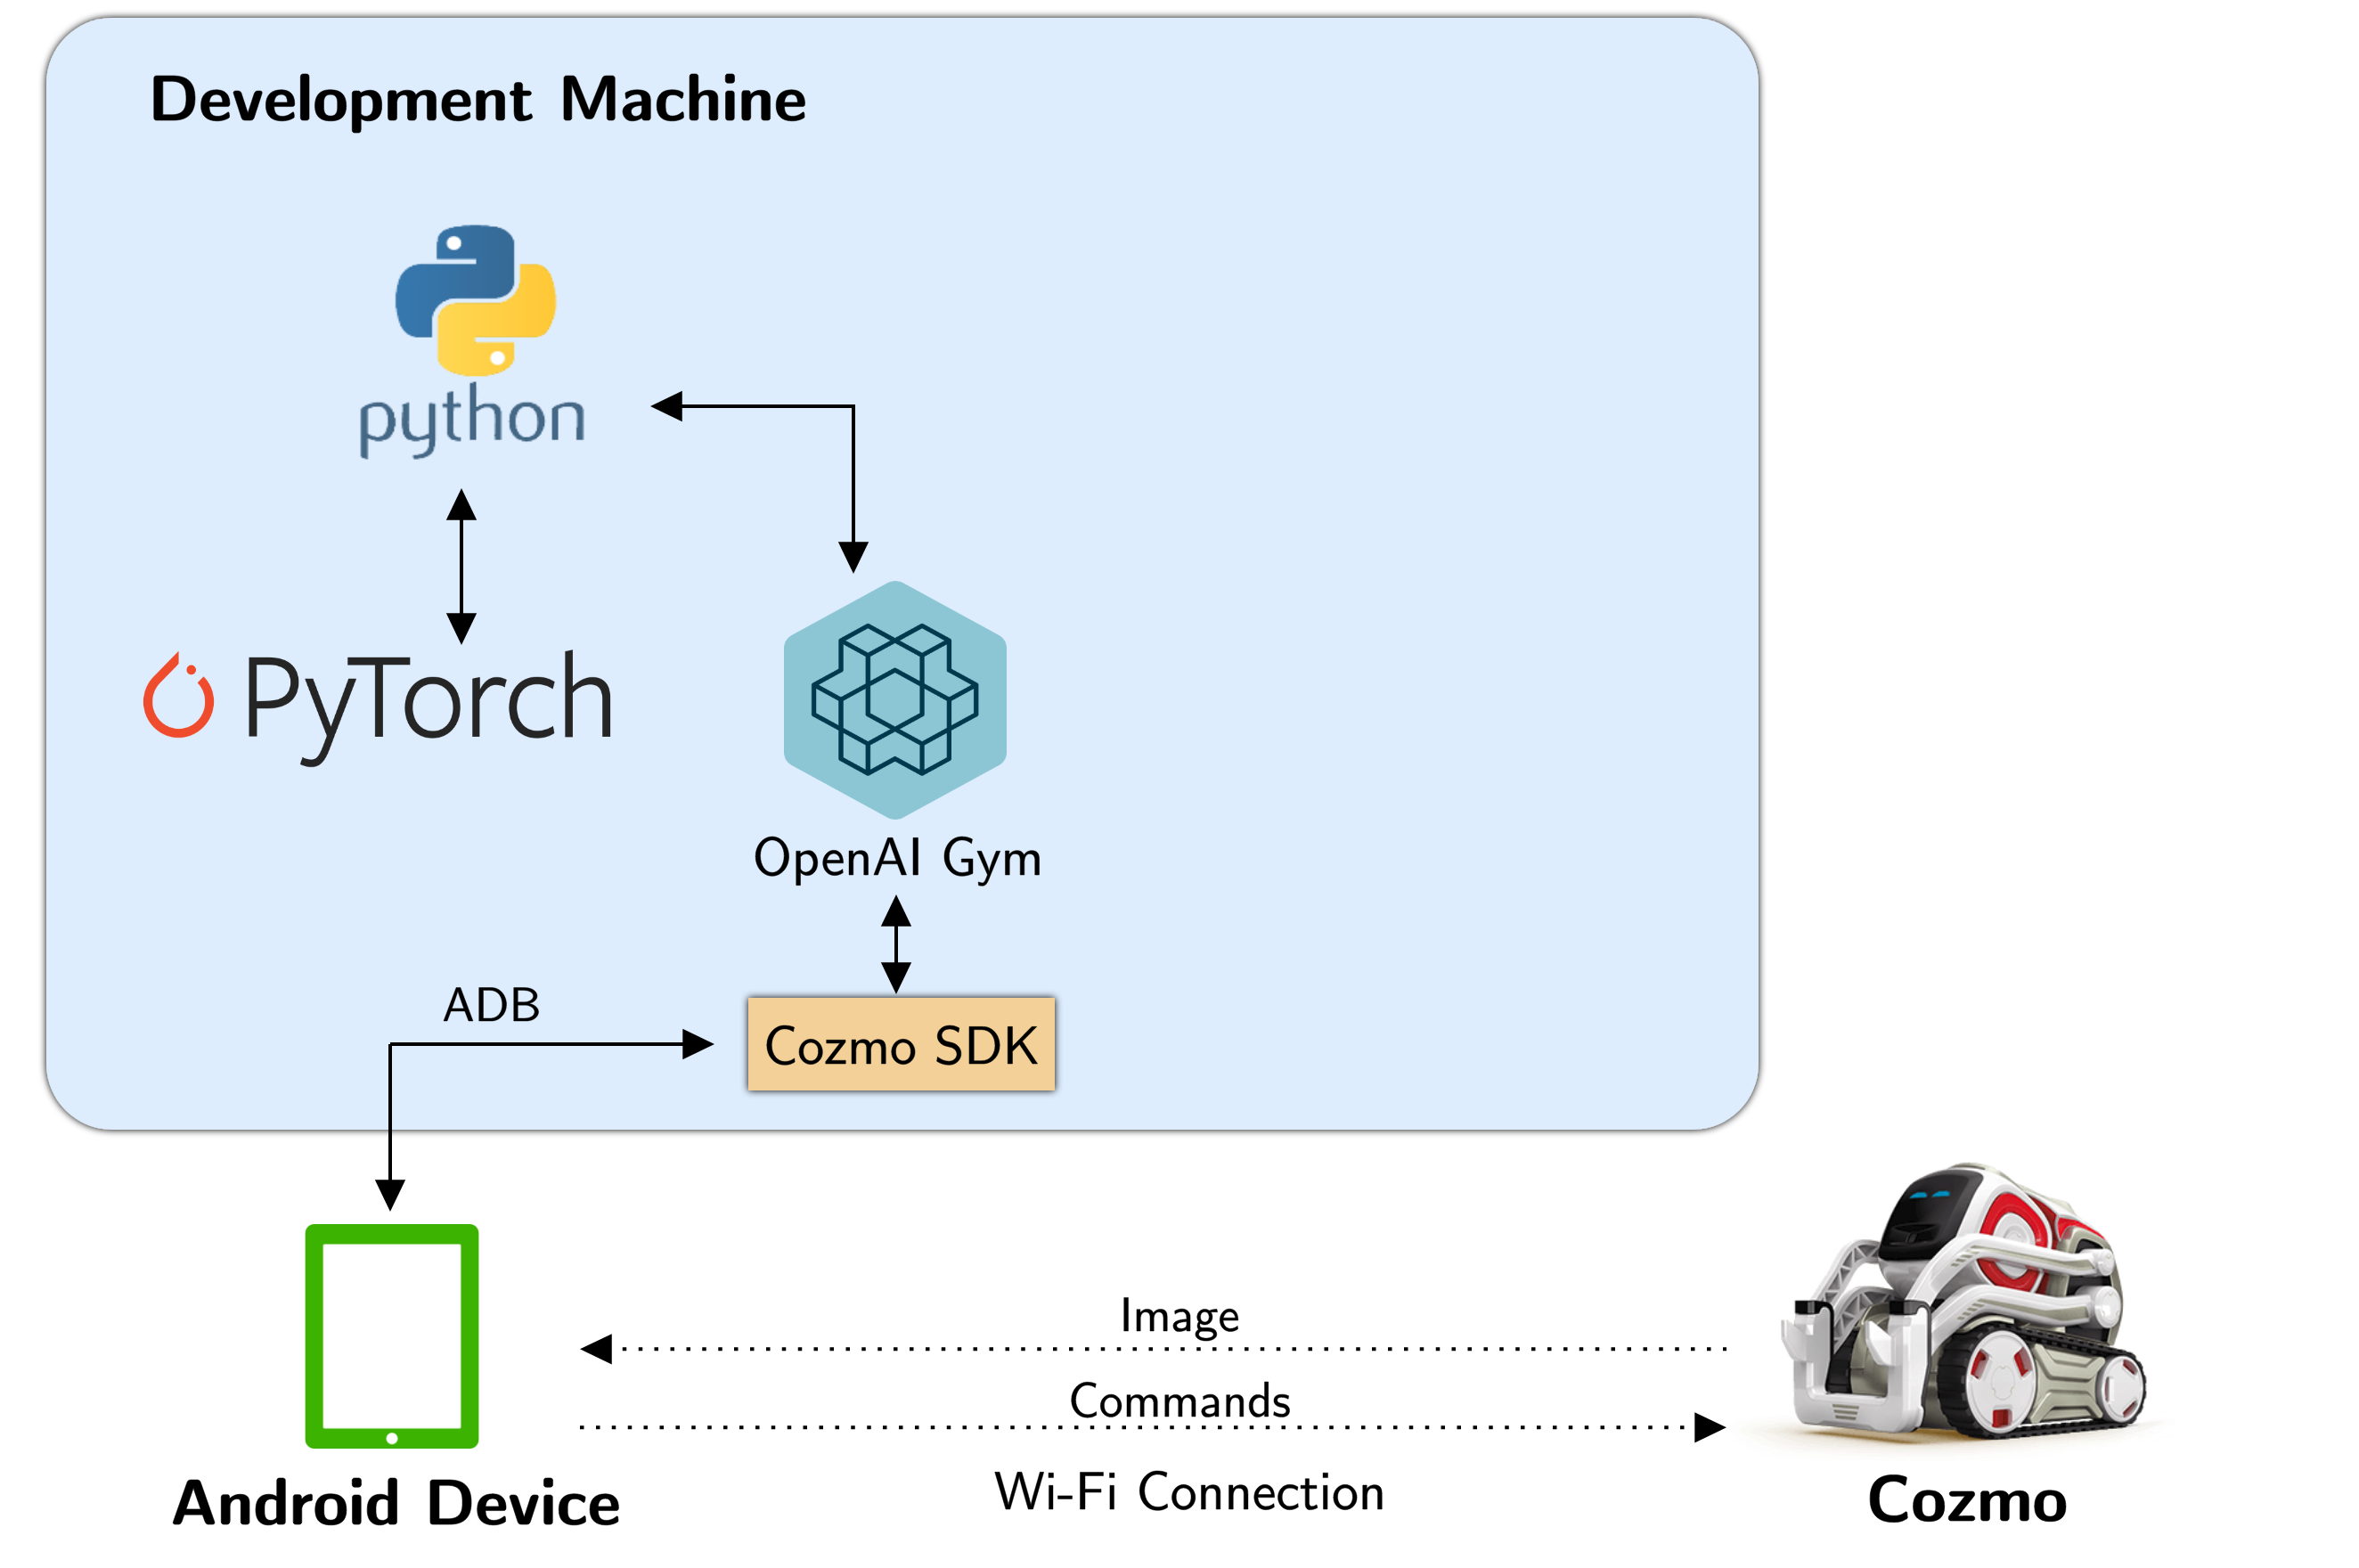
\includegraphics[height=0.9\textheight]{img/cozmosys3.png}}

	\only<5>{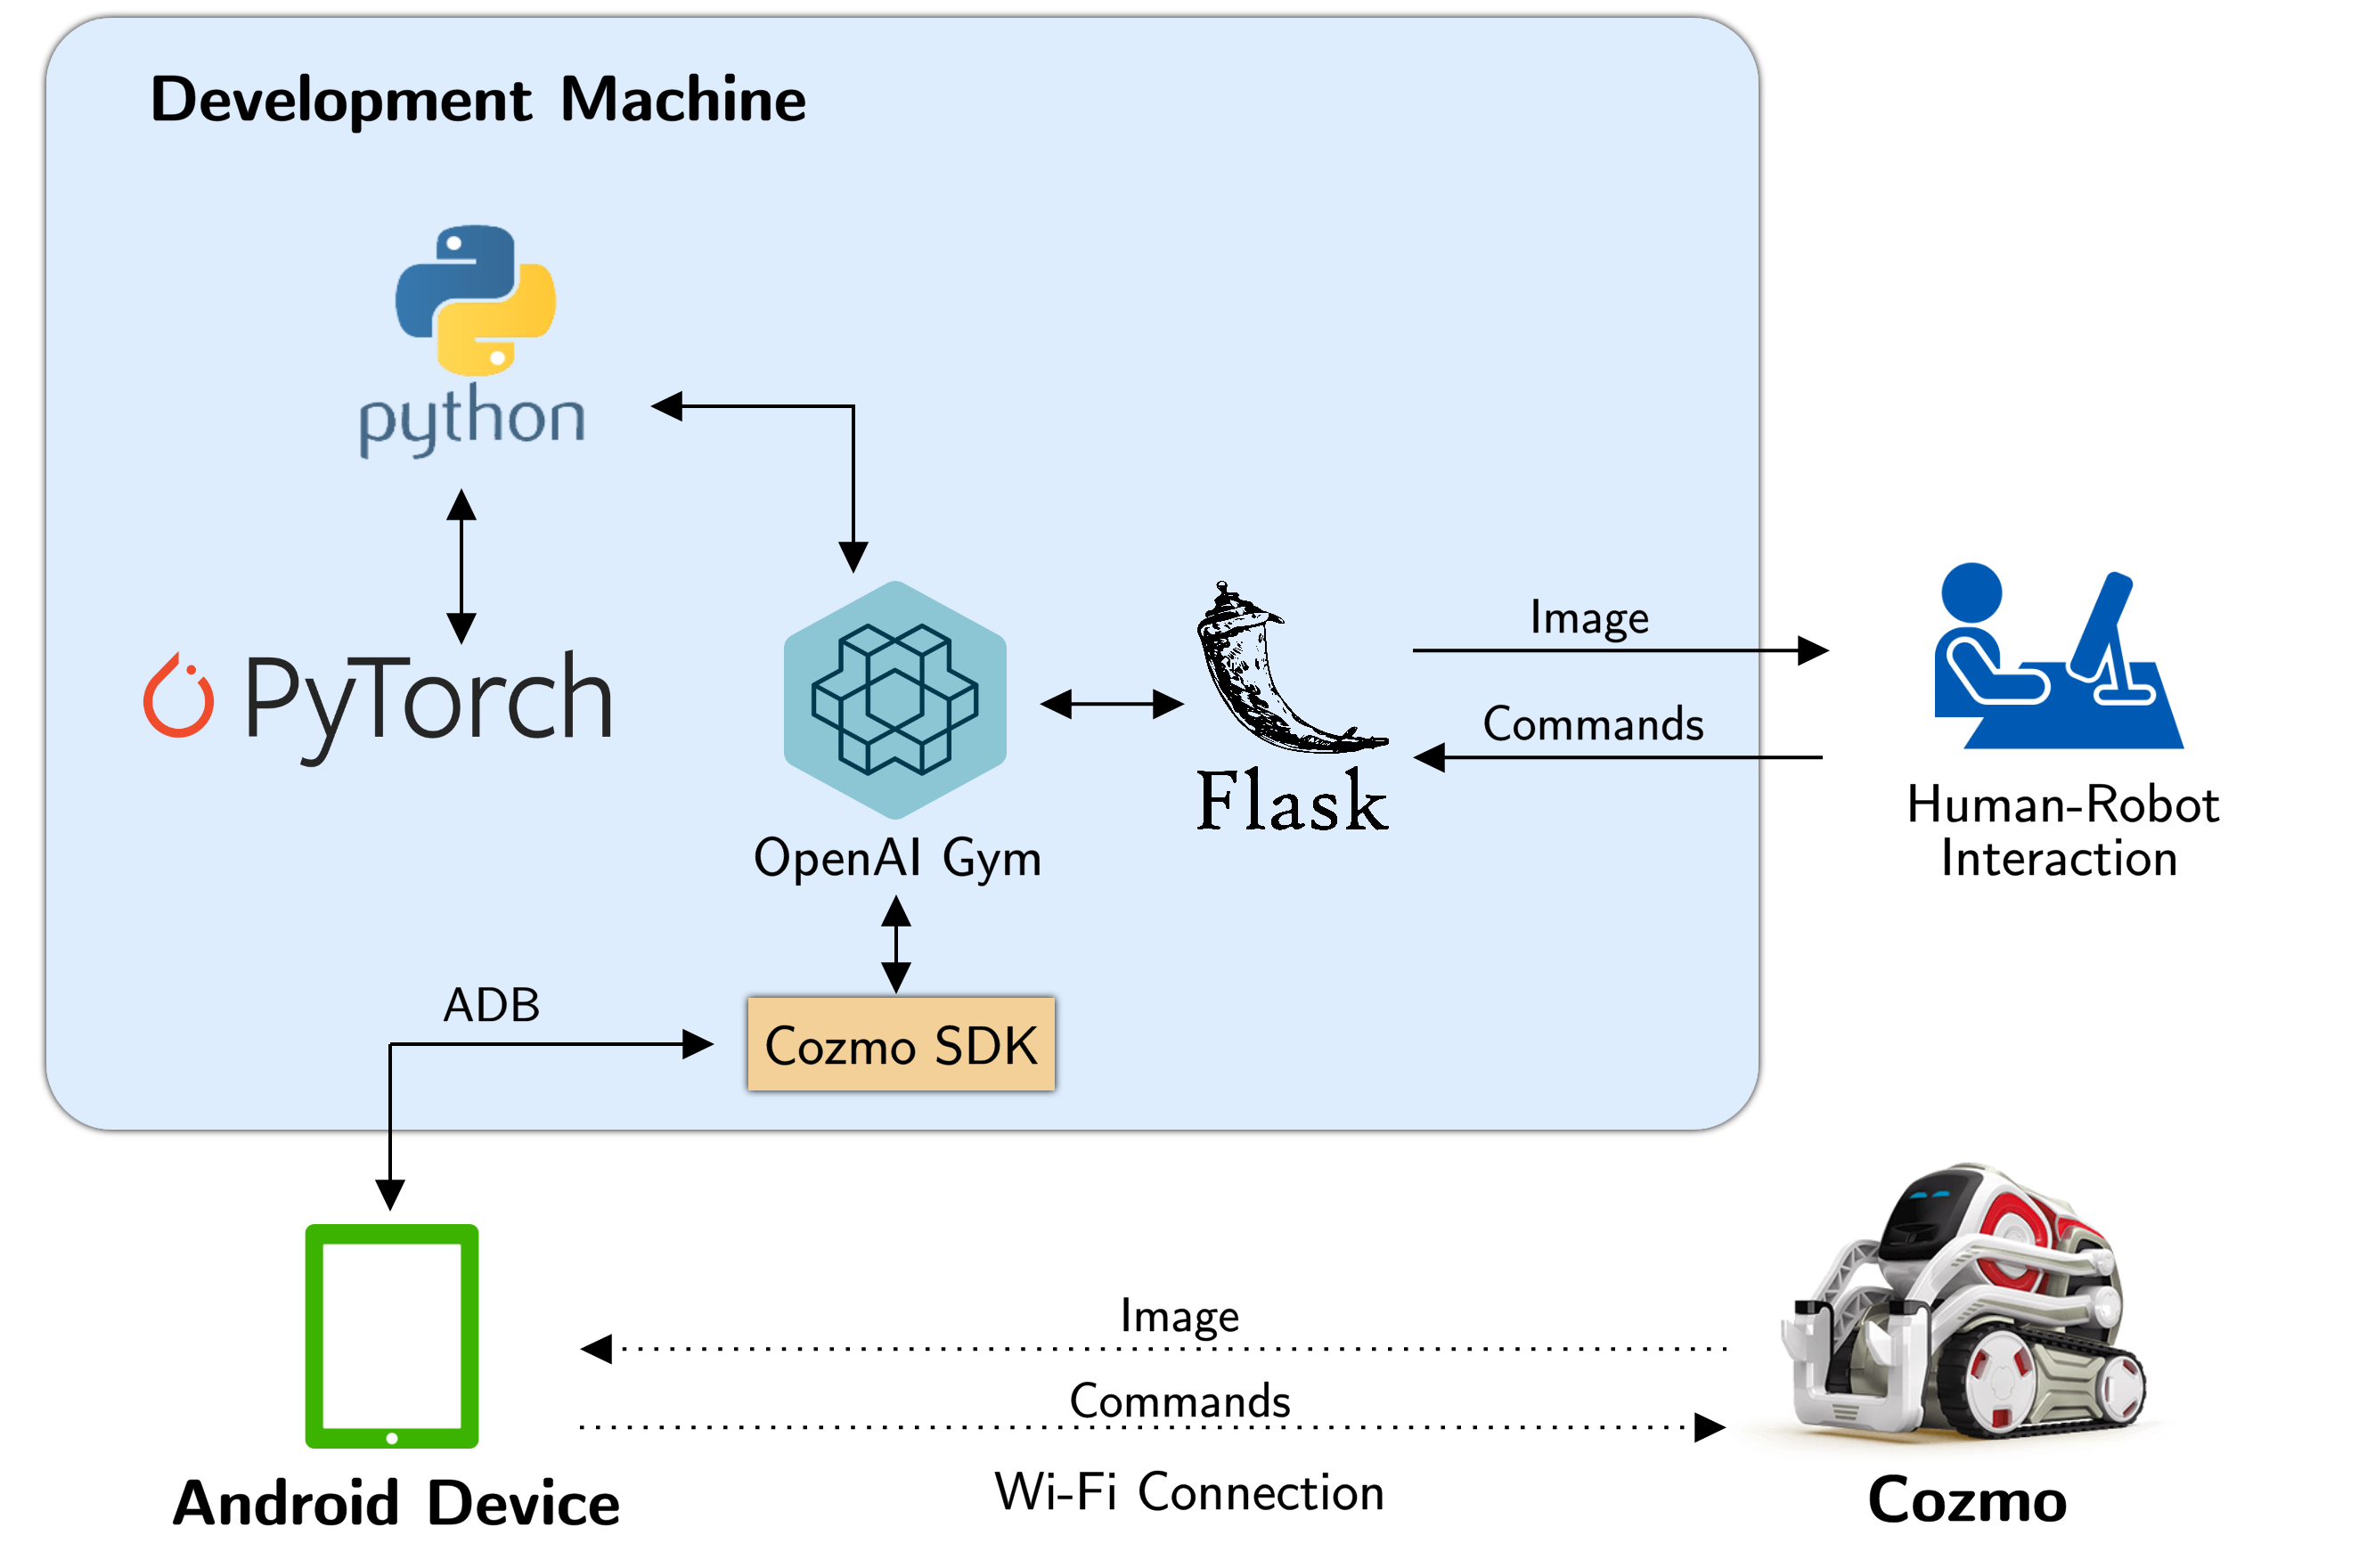
\includegraphics[height=0.9\textheight]{img/cozmosys4.png}}

	\only<6>{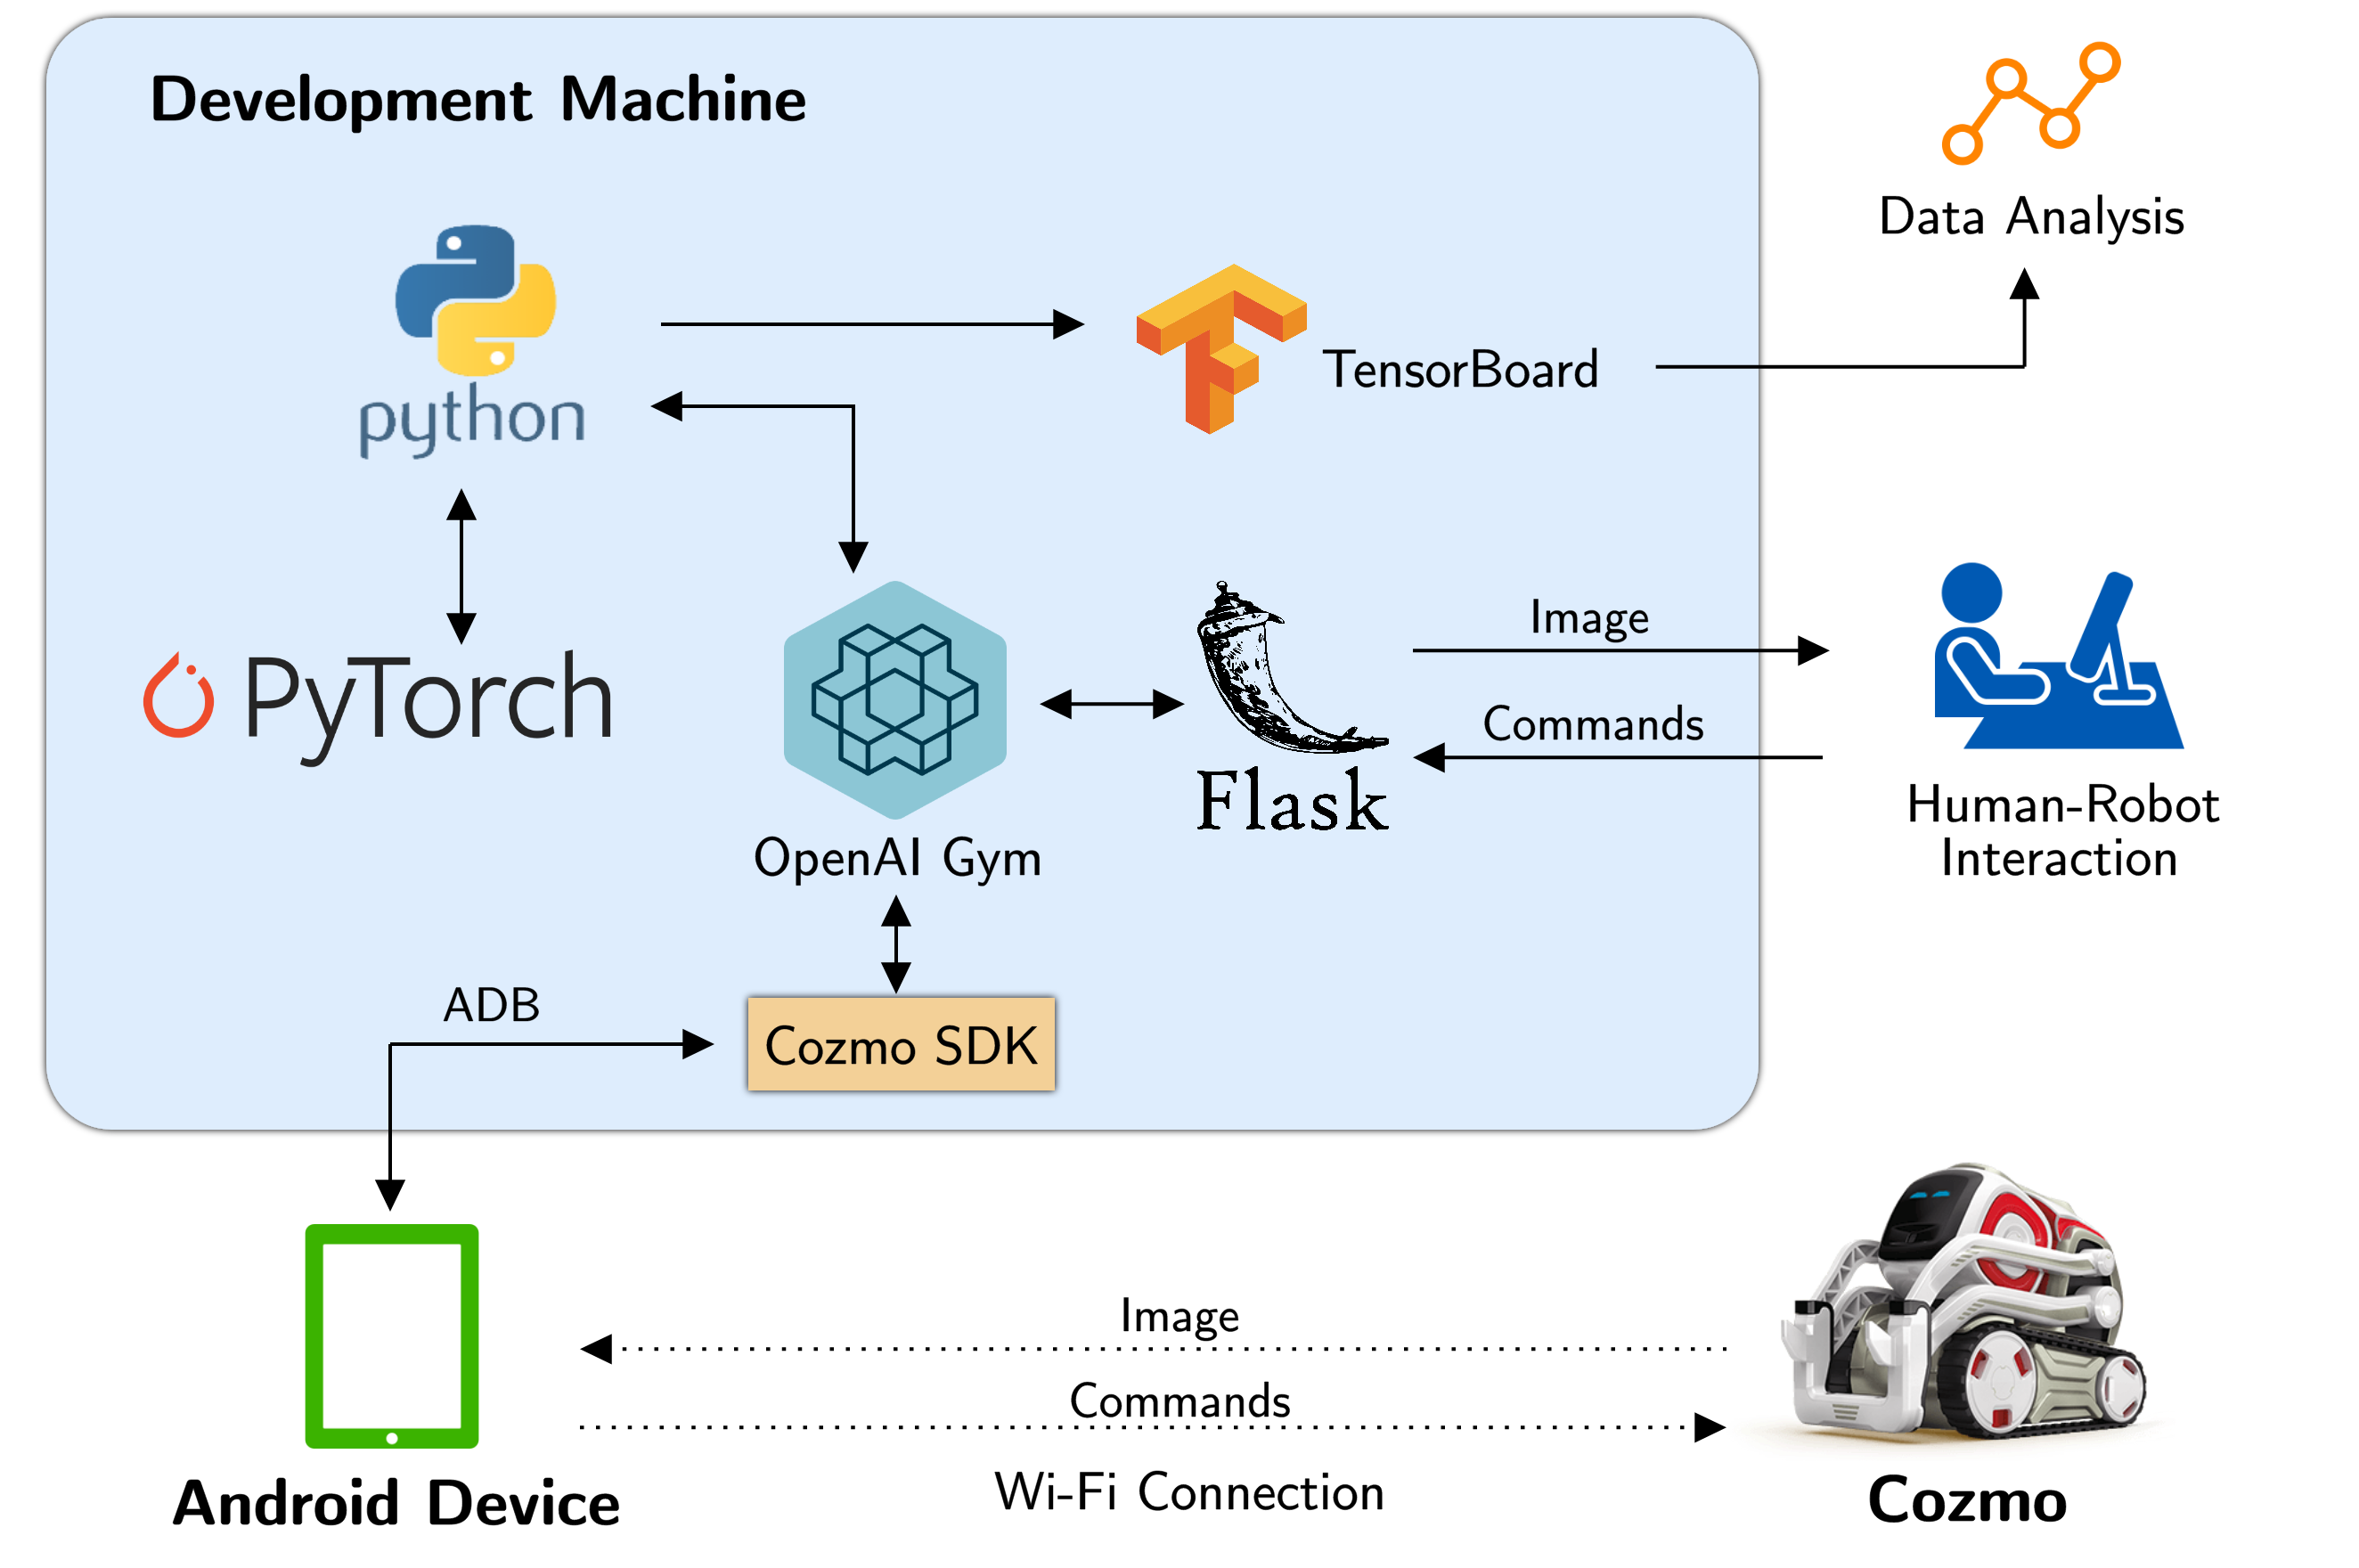
\includegraphics[height=0.9\textheight]{img/cozmosys6.png}}

\end{frame}

\begin{frame}{System Features}
	\begin{columns}
		\begin{column}{0.4\linewidth}
			\centering
			
\includegraphics[width=0.6\linewidth]{img/feature.png}
		\end{column}
		\begin{column}{0.6\linewidth}
			\begin{itemize}[<+- | alert@+>]
				\item Backup/Restore feature:
				      \begin{itemize}[<+- | alert@+>]
					      \item Episode restore
					      \item Checkpoint restore
				      \end{itemize}
				\item Playground Recording
			\end{itemize}
		\end{column}
	\end{columns}
\end{frame}



\sectiondark{Experimental methodology and results}

\begin{frame}{Hyper-parameters used}
	\centering
	TODO
\end{frame}

\begin{frame}{Convolutional Neural Network Architecture}
	\centering
	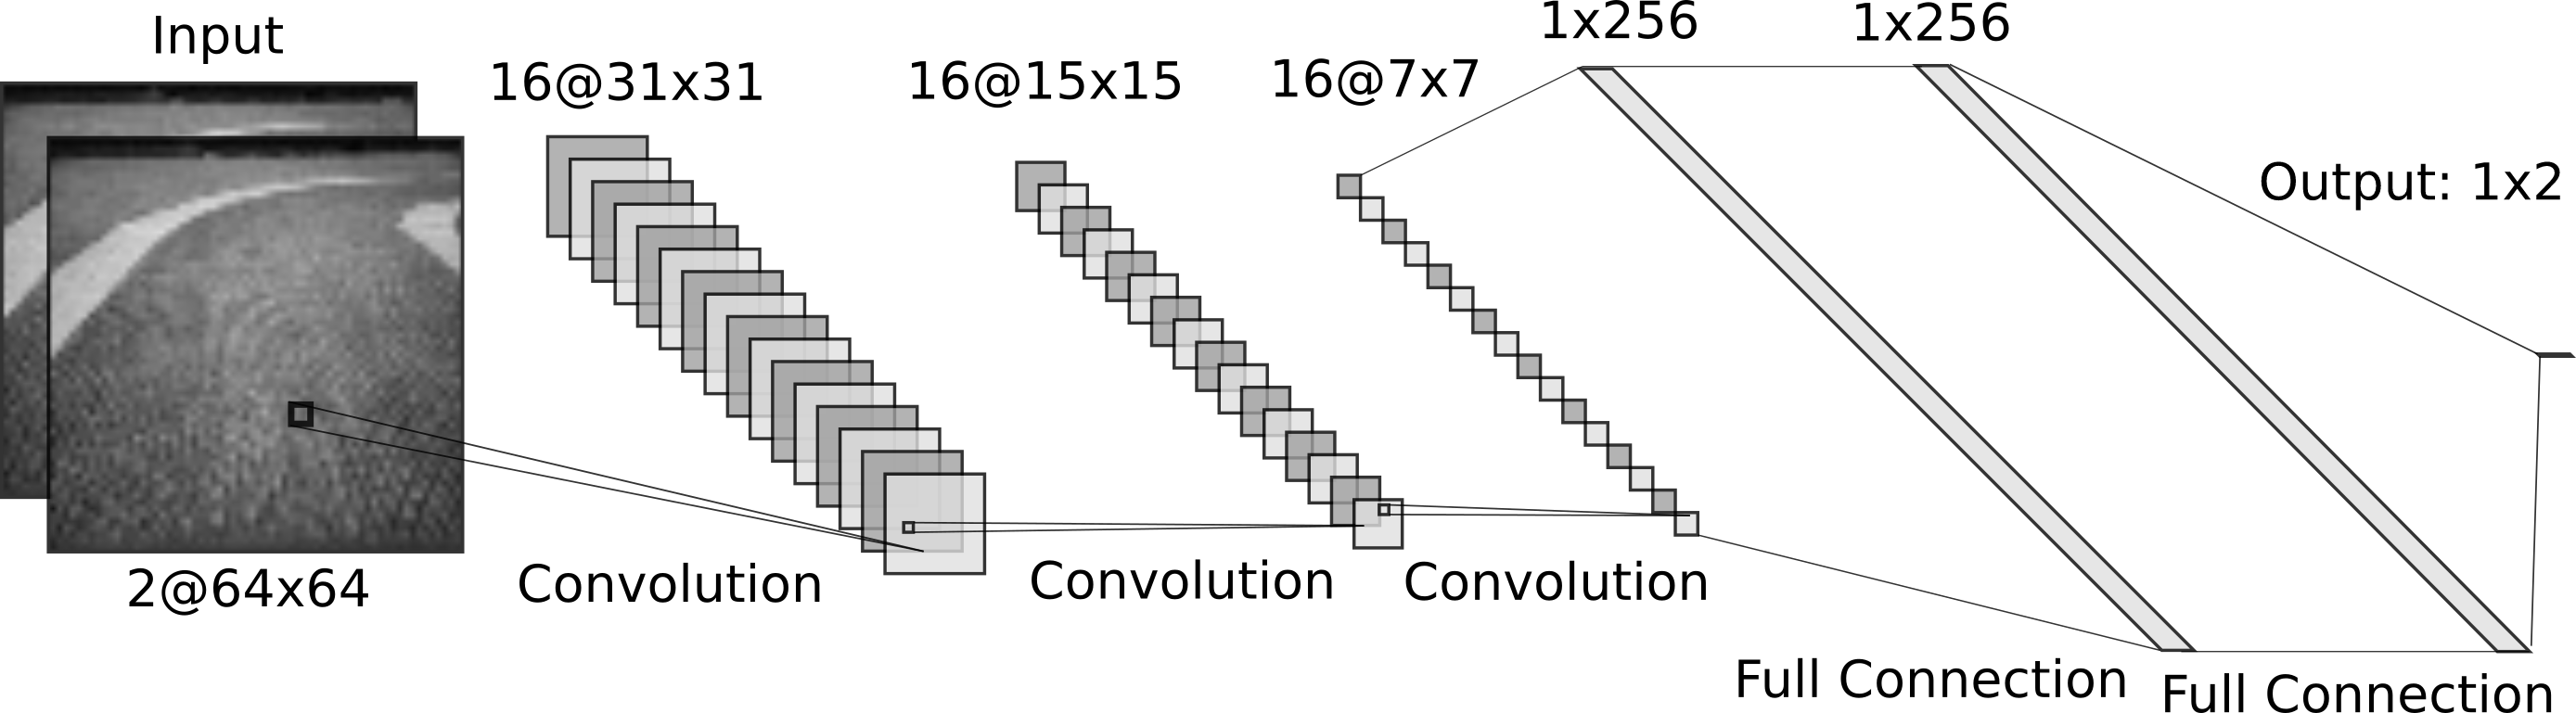
\includegraphics[width=0.9\textwidth]{img/cnn_cozmo.png}
	\begin{itemize}%[<+- | alert@+>]
		\item 3 Convolutional Layers: 16 features ($3\times3$), Stride 2, Padding 0
		\item 2 Fully Connected Layer with hidden size = 256
	\end{itemize}
\end{frame}

\begin{frame}{Pendulum-v0 DDPG Results}
	\begin{figure}[H]
		\centering
		\begin{tikzpicture}
			\begin{axis}[axis on top,
					width=0.8\textwidth,
					height=0.8\textheight,
					xmin=5000,
					xmax=50000,
					ymax=0,
					set layers=standard,
					cycle list name=test,
					grid=both,
					grid style={solid,gray!30!white},
					% axis lines=middle,
					xlabel=Epoch,
					ylabel style={align=center}, ylabel=Average Reward Value,
					%legend style={at={(0.99,0.3)},anchor=east},
					legend pos=south east,
					% extra y ticks = {90},
					%     extra y tick style={grid=major, grid style={solid,green},y tick label style={
					%         /pgf/number format/.cd,precision=10
					%}},
					% x label style={at={(axis description cs:0.5,0)},anchor=north},
					%y label style={at={(axis description cs:-0.1,.5)},rotate=90,anchor=south}
				]

				\addplot table[x=Step,y=Mean, col sep=comma] {plots/pendulum/ddpg_pendulum_test.csv};
				%\addlegendentry{Mean Reward of last 100 episode};

				\addplot [name path=upper,draw=none, forget plot] table[x=Step,y expr=\thisrow{Max}, col sep=comma] {plots/pendulum/ddpg_pendulum_test.csv};

				\addplot [name path=lower,draw=none, forget plot] table[x=Step,y expr=\thisrow{Min}, col sep=comma] {plots/pendulum/ddpg_pendulum_test.csv};

				\addplot [fill=test_color_3] fill between[of=upper and lower];

				\addplot [name path=upper1,draw=none, forget plot] table[x=Step,y expr=\thisrow{Mean}+\thisrow{StDev}, col sep=comma] {plots/pendulum/ddpg_pendulum_test.csv};

				\addplot [name path=lower1,draw=none, forget plot] table[x=Step,y expr=\thisrow{Mean}-\thisrow{StDev}, col sep=comma] {plots/pendulum/ddpg_pendulum_test.csv};

				\addplot [fill=test_color_2] fill between[of=upper1 and lower1];

				\addlegendentry{Mean $\mu$};
				\addlegendentry{Area $[min, max]$};
				\addlegendentry{Area $[\mu-\sigma, \mu+\sigma]$};

			\end{axis}
		\end{tikzpicture}
		\caption[DDPG Pendulum-v0 Test Average Reward Plot]{DDPG Pendulum-v0 Test Average Reward Plot.}
		\label{fig:ddpg_pendulum_test_reward}
	\end{figure}
	\note{
		The graph reports mean, standard deviation range and min-max range of the average reward obtained from 10 test episodes every 5000 epochs.
		They are calculated on 10 runs with different seeds.}
\end{frame}

\begin{frame}{Pendulum-v0 SAC Results}
	\begin{figure}[H]
		\centering
		\begin{tikzpicture}
			\begin{axis}[axis on top,
					width=0.8\textwidth,
					height=0.8\textheight,
					xmin=5000,
					xmax=50000,
					ymax=0,
					set layers=standard,
					cycle list name=test,
					grid=both,
					grid style={solid,gray!30!white},
					% axis lines=middle,
					xlabel=Epoch,
					ylabel style={align=center}, ylabel=Average Reward Value,
					%legend style={at={(0.99,0.3)},anchor=east},
					legend pos=south east,
					% extra y ticks = {90},
					%     extra y tick style={grid=major, grid style={solid,green},y tick label style={
					%         /pgf/number format/.cd,precision=10
					%}},
					% x label style={at={(axis description cs:0.5,0)},anchor=north},
					%y label style={at={(axis description cs:-0.1,.5)},rotate=90,anchor=south}
				]

				\addplot table[x=Step,y=Mean, col sep=comma] {plots/pendulum/sac_pendulum_test.csv};
				%\addlegendentry{Mean Reward of last 100 episode};

				\addplot [name path=upper,draw=none, forget plot] table[x=Step,y expr=\thisrow{Max}, col sep=comma] {plots/pendulum/sac_pendulum_test.csv};

				\addplot [name path=lower,draw=none, forget plot] table[x=Step,y expr=\thisrow{Min}, col sep=comma] {plots/pendulum/sac_pendulum_test.csv};

				\addplot [fill=test_color_3] fill between[of=upper and lower];

				\addplot [name path=upper1,draw=none, forget plot] table[x=Step,y expr=\thisrow{Mean}+\thisrow{StDev}, col sep=comma] {plots/pendulum/sac_pendulum_test.csv};

				\addplot [name path=lower1,draw=none, forget plot] table[x=Step,y expr=\thisrow{Mean}-\thisrow{StDev}, col sep=comma] {plots/pendulum/sac_pendulum_test.csv};

				\addplot [fill=test_color_2] fill between[of=upper1 and lower1];

				\addlegendentry{Mean $\mu$};
				\addlegendentry{Area $[min, max]$};
				\addlegendentry{Area $[\mu-\sigma, \mu+\sigma]$};

			\end{axis}
		\end{tikzpicture}
		\caption[SAC Pendulum-v0 Test Average Reward Plot]{SAC Pendulum-v0 Test Average Reward Plot.}
		\label{fig:sac_pendulum_test_reward}
	\end{figure}
	\note{
		The graph reports mean, standard deviation range and min-max range of the average reward obtained from 10 test episodes every 5000 epochs.
		They are calculated on 10 runs with different seeds.}
\end{frame}

\begin{frame}{CozmoDriver-v0 SAC Training}
	\centering
	\begin{figure}[!h]
		\centering
		\begin{tikzpicture}
			\begin{axis}[axis on top,
					enlargelimits=false,
					width=0.8\textwidth,
					height=0.8\textheight,
					xtick distance=500,
					set layers=standard,
					cycle list name=train,
					grid=both,
					grid style={solid,gray!30!white},
					% axis lines=middle,
					xlabel=Episode,
					ylabel style={align=center}, ylabel=Reward (mm),
					%legend style={at={(0.99,0.3)},anchor=east},
					legend pos=north west,
					% extra y ticks = {90},
					%     extra y tick style={grid=major, grid style={solid,green},y tick label style={
					%         /pgf/number format/.cd,precision=10
					%}},
					% x label style={at={(axis description cs:0.5,0)},anchor=north},
					%y label style={at={(axis description cs:-0.1,.5)},rotate=90,anchor=south}
				]

				\addplot table[x=Step,y=Value, col sep=comma] {plots/cozmo/sac_cozmo_train.csv};
				%\addlegendentry{Mean Reward of last 100 episode};

				\addlegendentry{Reward};

			\end{axis}
		\end{tikzpicture}
		\caption[SAC CozmoDriver-v0 Reward Plot]{SAC CozmoDriver-v0 Reward Plot.}
		\label{fig:sac_cozmo_reward}
	\end{figure}
\end{frame}

\begin{frame}{CozmoDriver-v0 SAC Training 100 average}
	\centering
	\begin{figure}[!h]
		\centering
		\begin{tikzpicture}
			\begin{axis}[axis on top,
					enlargelimits=false,
					width=0.8\textwidth,
					height=0.8\textheight,
					ymin=0,
					set layers=standard,
					xtick distance=500,
					cycle list name=train,
					grid=both,
					grid style={solid,gray!30!white},
					% axis lines=middle,
					xlabel=Episode,
					ylabel style={align=center}, ylabel=Average Reward (mm),
					%legend style={at={(0.99,0.3)},anchor=east},
					legend pos=south east,
					% extra y ticks = {90},
					%     extra y tick style={grid=major, grid style={solid,green},y tick label style={
					%         /pgf/number format/.cd,precision=10
					%}},
					% x label style={at={(axis description cs:0.5,0)},anchor=north},
					%y label style={at={(axis description cs:-0.1,.5)},rotate=90,anchor=south}
				]

				\addplot table[x=Step,y=Value, col sep=comma] {plots/cozmo/sac_cozmo_last100.csv};
				%\addlegendentry{Mean Reward of last 100 episode};

				\addlegendentry{Last 100 average reward $\mu$};

			\end{axis}
		\end{tikzpicture}
		\caption[SAC CozmoDriver-v0 Last 100 Episode Average Reward Plot]{SAC CozmoDriver-v0 Last 100 Episode Average Reward Plot.}
		\label{fig:sac_cozmo_last100}
	\end{figure}
\end{frame}

\begin{frame}{CozmoDriver-v0 SAC Temperature}
	\centering
	\begin{figure}[!h]
		\centering
		\begin{tikzpicture}
		\begin{axis}[axis on top,
		width=0.8\textwidth,
		height=0.8\textheight,
		enlargelimits=false,
		set layers=standard,
		cycle list name=train,
		ymin=0,
		scaled x ticks=true,
		grid=both,
		grid style={solid,gray!30!white},
		% axis lines=middle,
		xlabel=Epoch,
		ylabel style={align=center}, ylabel=Temperature Value ($\alpha$),
		%legend style={at={(0.99,0.3)},anchor=east},
		legend pos=south east,
		% extra y ticks = {90},
		%     extra y tick style={grid=major, grid style={solid,green},y tick label style={
		%         /pgf/number format/.cd,precision=10
		%}},
		% x label style={at={(axis description cs:0.5,0)},anchor=north},
		%y label style={at={(axis description cs:-0.1,.5)},rotate=90,anchor=south}
		]
		
		\addplot table[x=Step,y=Value, col sep=comma] {plots/cozmo/sac_cozmo_temperature.csv};
		%\addlegendentry{Mean Reward of last 100 episode};
		
		
		\addlegendentry{Temperature $\alpha$};
		
		\end{axis}
		\end{tikzpicture}
		\caption[SAC CozmoDriver-v0 auto-tuned temperature]{SAC Pendulum-v0 auto-tuned temperature.}
		\label{fig:sac_cozmo_temperature}
	\end{figure}
	
\end{frame}

\begin{frame}{CozmoDriver-v0 SAC Test}
	%%%%%%%%%%%%%%%%%%%%%%
	%
	% TEST PLOTS
	%
	%%%%%%%%%%%%%%%%%%%%%%

	\begin{figure}[!h]
		\centering
		\begin{tikzpicture}
			\begin{axis}[axis on top,
					scaled ticks=true,
					enlargelimits=false,
					width=0.8\textwidth,
					height=0.8\textheight,
					ymin=0,
					set layers=standard,
					cycle list name=test,
					grid=both,
					grid style={solid,gray!30!white},
					% axis lines=middle,
					xlabel=Epoch,
					ylabel style={align=center}, ylabel=Reward (mm),
					%legend style={at={(0.99,0.3)},anchor=east},
					legend pos=north west,
					% extra y ticks = {90},
					%     extra y tick style={grid=major, grid style={solid,green},y tick label style={
					%         /pgf/number format/.cd,precision=10
					%}},
					% x label style={at={(axis description cs:0.5,0)},anchor=north},
					%y label style={at={(axis description cs:-0.1,.5)},rotate=90,anchor=south}
				]

				\addplot table[x=Step,y=Mean, col sep=comma] {plots/cozmo/sac_cozmo_test.csv};
				%\addlegendentry{Mean Reward of last 100 episode};

				\addplot [name path=upper,draw=none, forget plot] table[x=Step,y expr=\thisrow{Max}, col sep=comma] {plots/cozmo/sac_cozmo_test.csv};

				\addplot [name path=lower,draw=none, forget plot] table[x=Step,y expr=\thisrow{Min}, col sep=comma] {plots/cozmo/sac_cozmo_test.csv};

				\addplot [fill=test_color_3] fill between[of=upper and lower];

				\addplot [name path=upper1,draw=none, forget plot] table[x=Step,y expr=\thisrow{Mean}+\thisrow{StDev}, col sep=comma] {plots/cozmo/sac_cozmo_test.csv};

				\addplot [name path=lower1,draw=none, forget plot] table[x=Step,y expr=\thisrow{Mean}-\thisrow{StDev}, col sep=comma] {plots/cozmo/sac_cozmo_test.csv};

				\addplot [fill=test_color_2] fill between[of=upper1 and lower1];

				\addlegendentry{Mean $\mu$};
				\addlegendentry{Area $[min, max]$};
				\addlegendentry{Area $[\mu-\sigma, \mu+\sigma]$};

			\end{axis}
		\end{tikzpicture}
		\caption[SAC CozmoDriver-v0 Test Reward Plot]{SAC CozmoDriver-v0 Test Reward Plot.}
		\label{fig:sac_cozmo_test}
	\end{figure}
\end{frame}
\begin{frame}{CozmoDriver-v0 SAC Test Mean}
	%%%%%%%%%%%%%%%%%%%%%%
	%
	% TEST PLOTS
	%
	%%%%%%%%%%%%%%%%%%%%%%

	\begin{figure}[!h]
		\centering
		\begin{tikzpicture}
			\begin{axis}[axis on top,
					scaled ticks=true,
					enlargelimits=false,
					width=0.8\textwidth,
					height=0.8\textheight,
					ymin=0,
					set layers=standard,
					cycle list name=test,
					grid=both,
					grid style={solid,gray!30!white},
					% axis lines=middle,
					xlabel=Epoch,
					ylabel style={align=center}, ylabel=Reward (mm),
					%legend style={at={(0.99,0.3)},anchor=east},
					legend pos=north west,
					% extra y ticks = {90},
					%     extra y tick style={grid=major, grid style={solid,green},y tick label style={
					%         /pgf/number format/.cd,precision=10
					%}},
					% x label style={at={(axis description cs:0.5,0)},anchor=north},
					%y label style={at={(axis description cs:-0.1,.5)},rotate=90,anchor=south}
				]

				\addplot table[x=Step,y=Mean, col sep=comma] {plots/cozmo/sac_cozmo_test.csv};
				%\addlegendentry{Mean Reward of last 100 episode};

				\addlegendentry{Mean $\mu$};
			\end{axis}
		\end{tikzpicture}
		\caption[SAC CozmoDriver-v0 Test Average Reward Plot]{SAC CozmoDriver-v0 Test Average Reward Plot.}
		\label{fig:sac_cozmo_test_mean}
	\end{figure}
\end{frame}

\begin{frame}{Episode Showcase - 1}
	\centering
	%\href{run:/usr/bin/vlc ./video/epi2748.mp4}{Start Video}
	\animategraphics[loop,controls,width=0.4\linewidth]{15}{video/try/epi1-}{0}{251}
\end{frame}

\begin{frame}{Episode Showcase - 2}
	\centering
	%\href{run:/usr/bin/vlc ./video/epi2748.mp4}{Start Video}
	\animategraphics[loop,controls,width=0.4\linewidth]{15}{video/try/epi2-}{0}{255}
\end{frame}

\sectiondark{Conclusions and future work}

\begin{frame}{Conclusions}

	\begin{columns}
		\begin{column}{0.4\linewidth}
			\centering
			
\includegraphics[width=0.6\linewidth]{img/conclusion.png}
		\end{column}
		\begin{column}{0.6\linewidth}
			\begin{itemize}[<+- | alert@+>]
				\item Promising approach:
				      \begin{itemize}
					      \item \textbf{Maximum reward reached}: $\sim 3.5$ meters
					      \item Visible improvements during experiments
				      \end{itemize}
				\item Unstable for concrete application:
				      \begin{itemize}
					      \item \textbf{Average reward reached}: $\sim 1$ meter
					      \item It needs time to improve
				      \end{itemize}
			\end{itemize}
		\end{column}
	\end{columns}
\end{frame}

\begin{frame}{Future Work}
	\begin{columns}
		\begin{column}{0.4\linewidth}
			\centering
			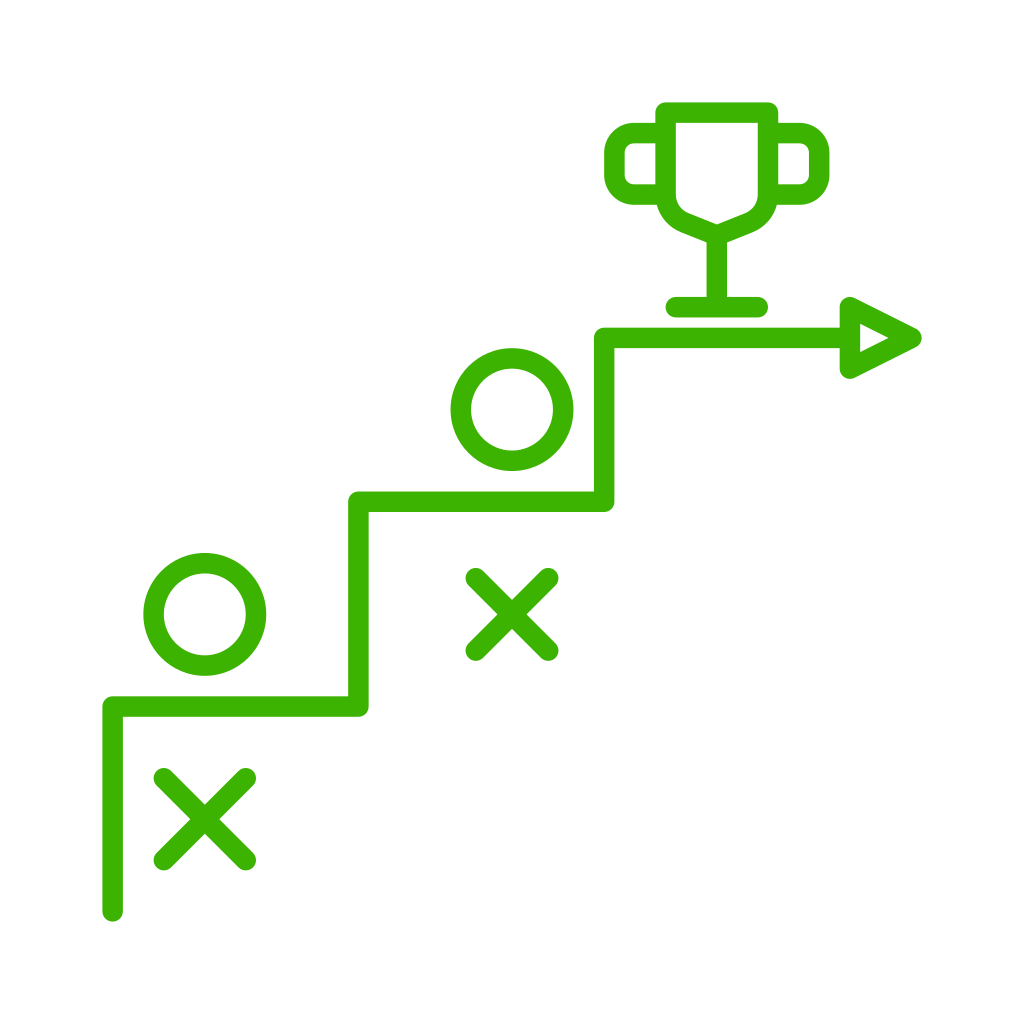
\includegraphics[width=0.6\linewidth]{img/future.png}
		\end{column}
		\begin{column}{0.6\linewidth}
			\begin{itemize}[<+- | alert@+>]
				\item Alternative Reward function analysis
				      \begin{itemize}
					      \item Penalise terminal high speed
				      \end{itemize}
				\item Improving Sensors
				      \begin{itemize}
					      \item Custom RC car (e.g.\ Donkey Car)
					      \item Anki Vector
				      \end{itemize}
				\item Feature Extraction
				      \begin{itemize}
					      \item Variational Auto-Encoder (VAE)
				      \end{itemize}
				\item Data fusion
				\item Model-based approach
			\end{itemize}
		\end{column}
	\end{columns}
\end{frame}



%\begin{frame}{Reinforcement Learning Example}
%	
%	\onslide<1->{Problems involving a \alert{\textbf{Human}} interacting with \alert{\textbf{Earth}}, which provides \textbf{material reward}.}
%	\onslide<2->{}	\onslide<3->{}
%	
%\textbf{Goal}: Accumulate money for his/her future
%	\begin{center}
%		\scalebox{0.9}{
%			\begin{tikzpicture}
%			% node Agent
%			\node[punkt] (agent) {Human};
%			% node Environment
%			\node[punkt, below=1cm of agent] (env) {Earth};
%			% node a_t
%			\node<1-1>[mylabel, below right=0.25cm and 0.5cm of agent] (action) {Study};
%			\node<2-2>[mylabel, below right=0.25cm and 0.5cm of agent] (action) {Work};
%			\node<3-3>[mylabel, below right=0.25cm and 1.25cm of agent] (action) {Rob a Bank};
%			% node s_t
%			\node[mylabel, below left=-0.25cm and 1.75cm of agent] (state) {What the human sees and feels};
%			% node r_t
%			\node<1-1>[mylabel, below left=0.15cm and -1.1cm of agent] (reward) {$\{0,-10,10\}$€};			% node s_t+1
%			\node<2-2>[mylabel, below left=0.15cm and -1.1cm of agent] (reward) {$\{50,60\}$€};			% node s_t+1
%			\node<3-3>[mylabel, below left=0.15cm and -1.1cm of agent] (reward) {$100'000$€};			% node s_t+1
%			\node[mylabel, above left=-1.3cm and -1cm of env] (state) {};			% node r_t+1
%			\node[mylabel,above left=-.3cm and -1cm of env] (reward1) {};
%			\draw[pil]   (agent.east) -- ($(agent.east) + (1.2cm,0cm)$)  |-  (env.east);
%			\draw[pil]   ($(env.west) + (0,-0.2cm)$) -- ($(env.west) + (-1.2cm,-0.2cm)$);
%				\draw[pil]   ($(env.west) + (-1.2cm,-0.2cm)$) -- ($(env.west) + (-2cm,-0.2cm)$) |-($(agent.west) + (0,0.2cm)$);
%				\draw[pil]   ($(env.west) + (0,+0.2cm)$) -- ($(env.west) + (-1.2cm,+0.2cm)$);
%				\draw[pil]   ($(env.west) + (-1.2cm,+0.2cm)$) -- ($(env.west) + (-1.6cm,+0.2cm)$) |-($(agent.west) + (0,-0.2cm)$);
%				\draw[dashed]  ($(env.west) - (1.2cm,-0.5cm)$) -- ($(env.west) - (1.2cm,0.5cm)$);
%			\end{tikzpicture}
%		}
%	\end{center}
%	
%	
%\end{frame}




%
%\begin{frame}{The Reinforcement Learning Control System Stack}
%	\begin{itemize}
%		\item<1->{ Human Level Control through a WebApp (\textbf{Flask}, \textbf{Python} and \textbf{Javascript})}
%		\item<1->{Algorithm written in \textbf{Python}}
%		\item<1->{\textbf{PyTorch} as Deep Learning Framework}
%		\item<1->{\textbf{OpenAI Gym} Framework for Reinforcement Learning}
%		\item<1->{\textbf{Cozmo SDK}}
%	\end{itemize}
%\end{frame}
%
%\begin{frame}{Human Control Panel}
%	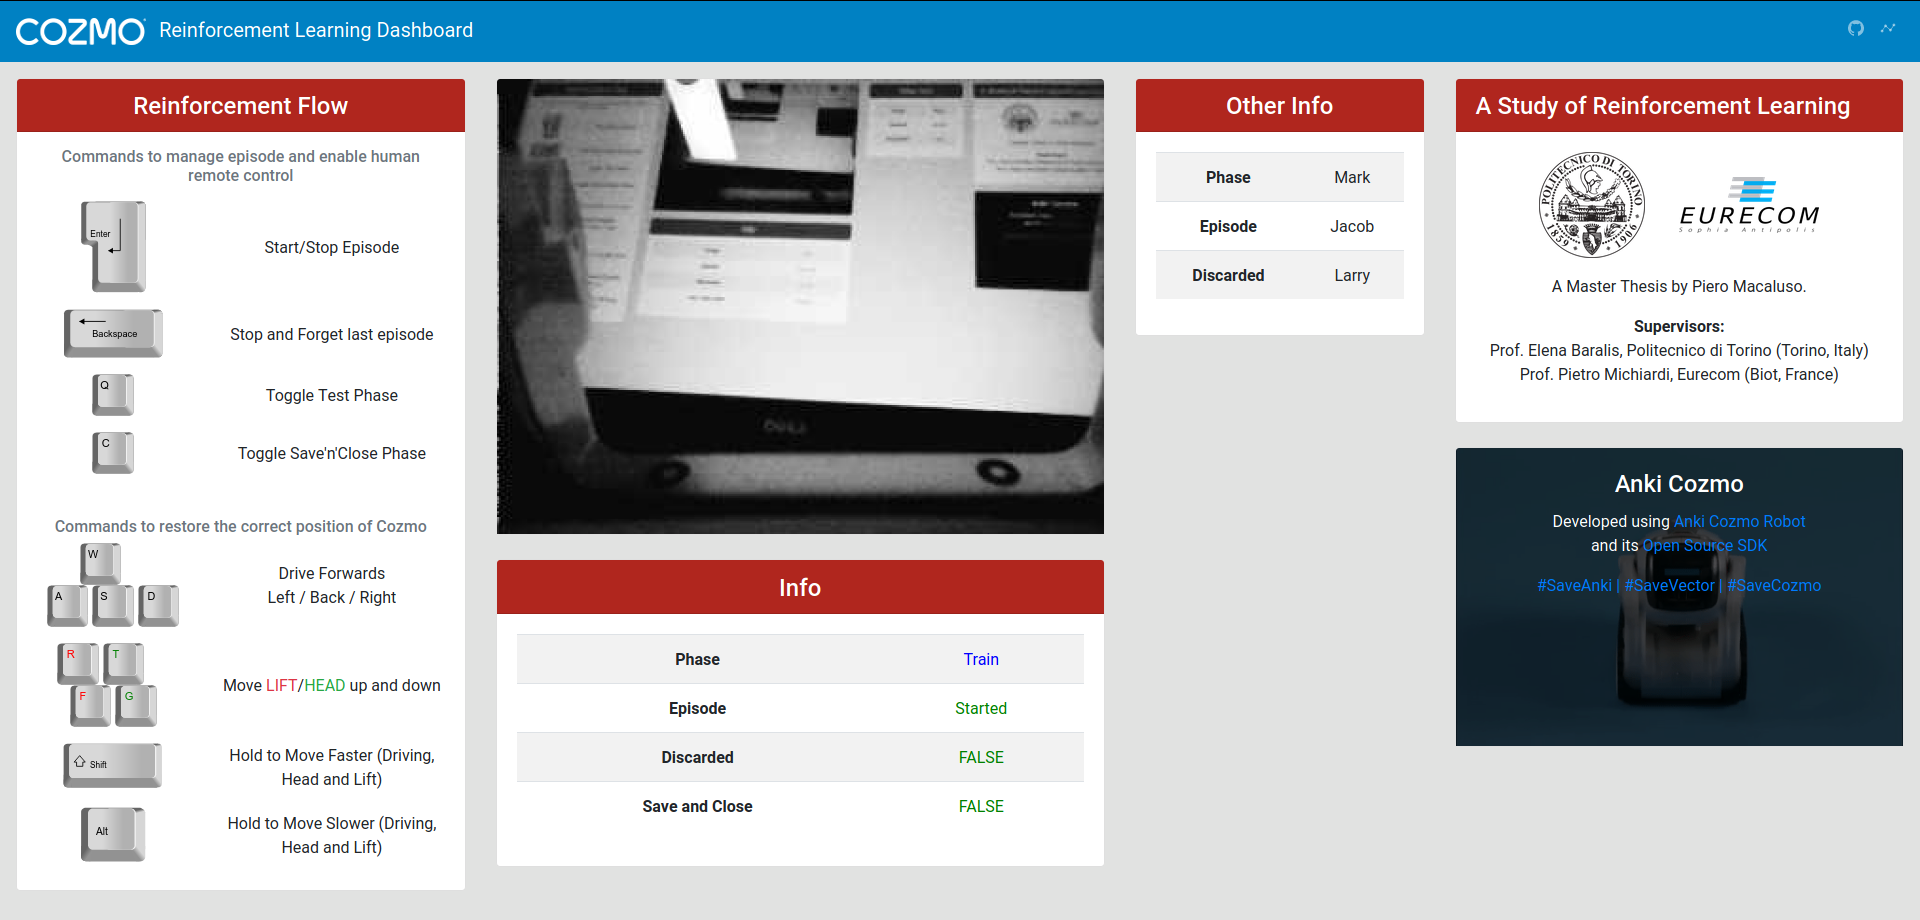
\includegraphics[width=1\linewidth]{img/dashboard.png}
%\end{frame}
%
%\begin{frame}{The Track}
%
%	\begin{columns}
%		\begin{column}{0.5\linewidth}
%			\begin{itemize}
%				\item<1->{Contrast between lane and asphalt.}
%				\item<1->{Lane width comparable to the real one.}
%				\item<1->{Fewer Reflections.}
%				\item<1->{Easily Repeatable.}
%			\end{itemize}
%		\end{column}
%		\begin{column}{0.5\linewidth}
%			\centering
%			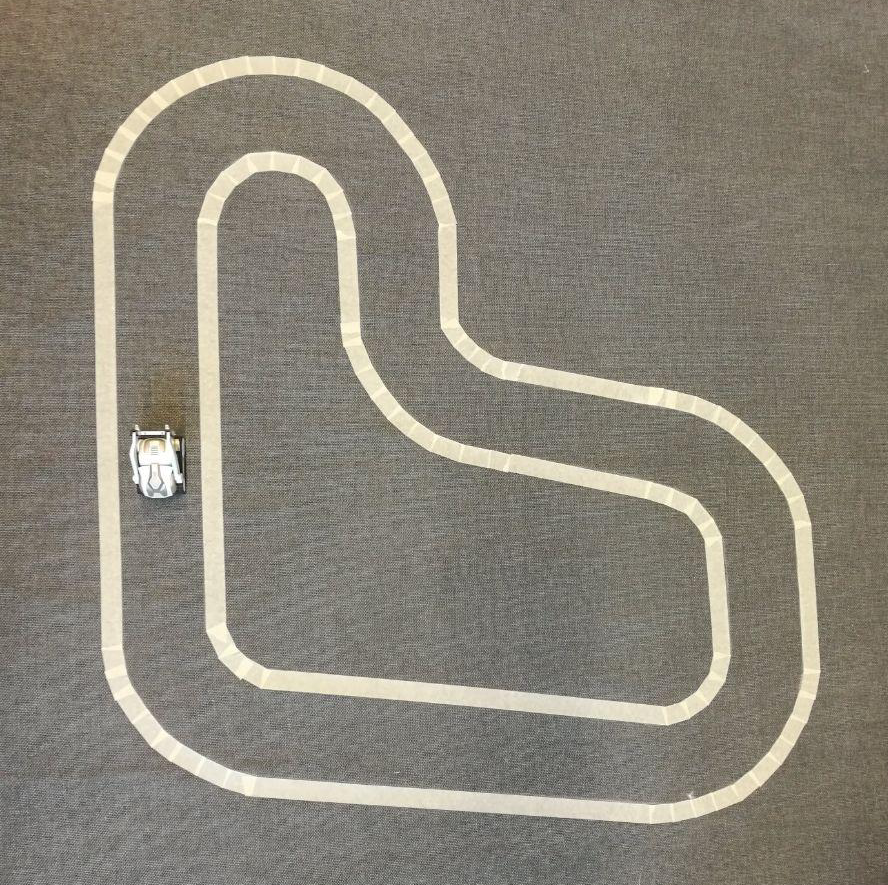
\includegraphics[width=0.9\linewidth]{img/track.png}
%		\end{column}
%	\end{columns}
%
%\end{frame}
%
%
%\begin{frame}{Considerations}
%	\centering
%	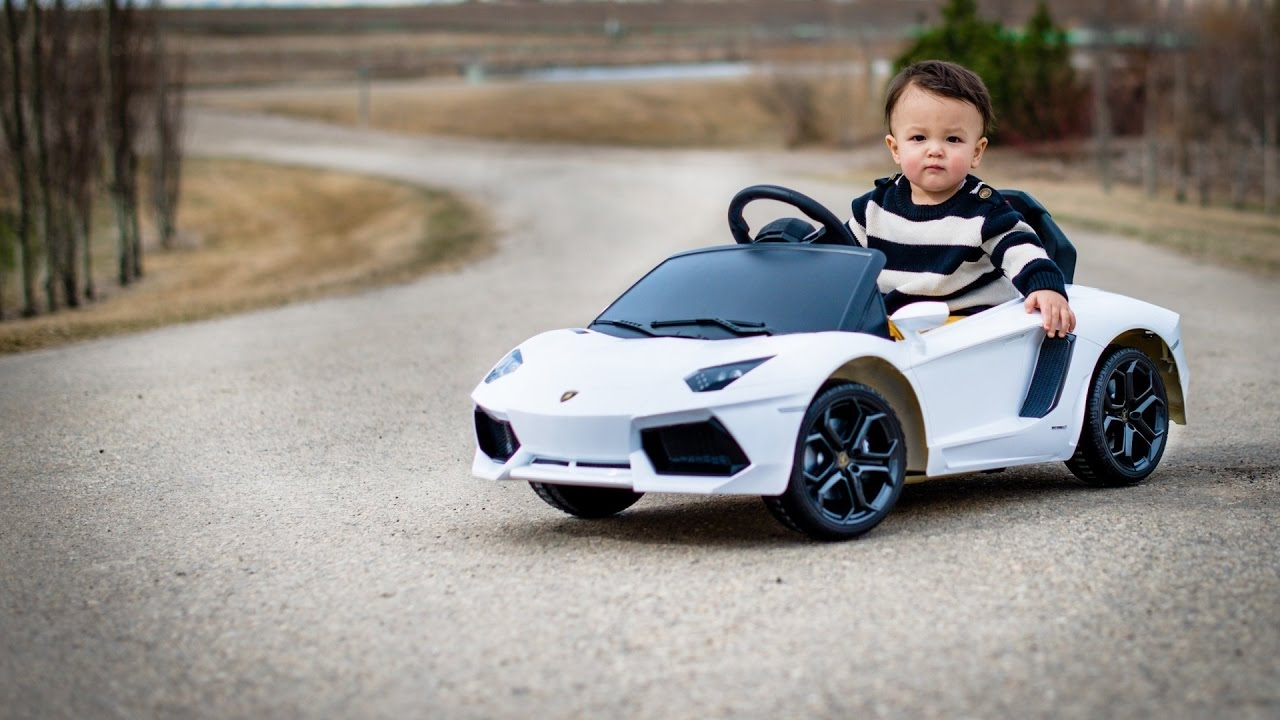
\includegraphics[width=0.5\linewidth]{img/baby.jpg}
%	\begin{itemize}
%		\item These results might appear not so extraordinary.
%		\item In reality, it is like teaching a \alert{\textbf{baby}} how to drive a car!
%		\item It is a process which starts from scratch. \textbf{From Zero to Hero!}
%	\end{itemize}
%\end{frame}
%
%%\begin{frame}{Best Episodes - Episode 2876}
%%	\centering
%%	\includemedia[
%%	addresource=video/episode_2876.mp4,
%%	activate=pageopen,transparent,
%%	passcontext,
%%	flashvars={source=video/episode_2876.mp4},
%%	width=0.8\linewidth, height=0.45\linewidth
%%	]{}{VPlayer.swf}%
%%\end{frame}
%
%\begin{frame}{Issues}
%	\begin{itemize}
%		\item Hunger for data.
%		\item Human Bias.
%		\item Narrow view of the camera.
%	\end{itemize}
%\end{frame}
%
%\begin{frame}{Possible improvements}
%	\begin{itemize}
%		\item Increase the number of epochs for each episode.
%		\item Apply gradient clipping.
%		\item Prioritized Experience Replay.
%		\item Improve Fault Recovery System.
%	\end{itemize}
%\end{frame}
%
%\begin{frame}{Possible developments}
%	\begin{itemize}
%		\item Increase the number of data (e.g\ sensors).
%		\item Overcome the limitations of Cozmo.
%		      \begin{itemize}
%			      \item Anki Vector
%			      \item Donkey Car
%		      \end{itemize}
%		\item Neural Network for object detection.
%	\end{itemize}
%\end{frame}

{\setbeamercolor{palette primary}{fg=white, bg=orange}
\begin{frame}[standout]
	Questions?
\end{frame}
}
\begin{frame}[standout]
	Thank you!
\end{frame}
\begin{frame}[allowframebreaks]{References}

	\printbibliography

\end{frame}

\appendix

\sectiondark{Appendix - Background}

\begin{frame}{Components of the Agent}
	\begin{itemize}
		\item{\textbf{Policy}:  agent’s behaviour function}
		      \begin{equation*}
			      \begin{aligned}
				      \text{\textbf{Deterministic}: } & \pi(s) = a                               \\
				      \text{\textbf{Stochastic}: }    & \pi(a|s) = \mathbb{P}[A_t = a | S_t = s]
			      \end{aligned}
		      \end{equation*}
		\item{\textbf{Value Function}:  policy evaluation function}
		      \begin{equation*}
			      \begin{aligned}
				      \text{\textbf{State Value}: }  & V^\pi(s) = \mathbb{E} \Bigg[\sum_{t \ge 0} \gamma^k r_t|s_0 = s, \pi\Bigg]                  \\
				      \text{\textbf{Action Value}: } & Q^\pi(s,a) = \mathbb{E} \Bigg[\sum_{t \ge 0} \gamma^k r_t \big| s_0 = s, a_0 = a, \pi\Bigg] \\
			      \end{aligned}
		      \end{equation*}
		\item{\textbf{Model}:  agent’s representation of the environment}
	\end{itemize}

\end{frame}


\begin{frame}{Model-Free Actor Critic methods}
	\begin{columns}
		\begin{column}{0.5\linewidth}
			\metroset{block=fill}
			\begin{exampleblock}{Critic Network}
				Estimates the value function. This could be the action value $Q$ or state value $V$.
			\end{exampleblock}
			\begin{exampleblock}{Actor Network}
				Updates the policy distribution in the direction suggested by the Critic (such as with policy gradients).
			\end{exampleblock}
		\end{column}
		\begin{column}{0.5\linewidth}
			\centering
			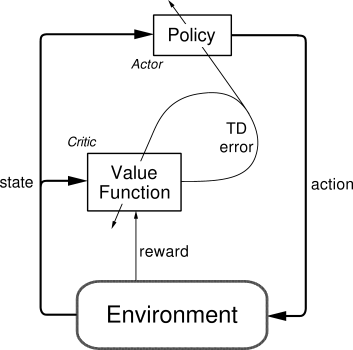
\includegraphics[width=0.8\linewidth]{img/actor_critic.png}
		\end{column}
	\end{columns}
	\footcite*{sutton2018reinforcement}

\end{frame}


\begin{frame}{Model-Free Actor Critic methods}
	\Large
	\begin{equation}\label{eq:tdlearning}
		V(s_t) \leftarrow V(s_t) + \alpha \big(\underbrace{\overbrace{r_{t+1} + \gamma V(s_{t+1})}^{\text{TD target}}- V(s_t)}_{\text{TD error} \ (\delta_t)}\big)
	\end{equation}
	\footcite*{sutton2018reinforcement}

\end{frame}

\begin{frame}{Categorizing Reinforcement Learning agents}
	\begin{columns}
		\begin{column}{0.5\linewidth}
			\begin{itemize}
				\item \textbf{Value Based}
				      \begin{itemize}
					      \item{\textcolor{lightgray}{No Policy (implicit)}}
					      \item{Value Function}
				      \end{itemize}
				\item \textbf{Policy Based}
				      \begin{itemize}
					      \item{Policy}
					      \item{\textcolor{lightgray}{No value function}}
				      \end{itemize}
				\item  \alert{\textbf{Actor Critic}}
				      \begin{itemize}
					      \item{Policy}
					      \item{Value function}
				      \end{itemize}
			\end{itemize}
		\end{column}
		\begin{column}{0.5\linewidth}
			\begin{itemize}
				\item \alert{\textbf{Model Free}}
				      \begin{itemize}
					      \item{Policy and/or value function}
					      \item{\textcolor{lightgray}{No Model}}
				      \end{itemize}
				\item \textbf{Model Based}
				      \begin{itemize}
					      \item{Policy and/or value function}
					      \item{Model}
				      \end{itemize}
			\end{itemize}
		\end{column}
	\end{columns}
\end{frame}

\begin{frame}{Deep Deterministic Policy Gradient (DDPG) - Neural Networks}
	\centering
	It uses \textbf{Target Networks} to minimise the instability MSBE loss
	\vspace{10mm}
	\begin{columns}
		\begin{column}{0.5\linewidth}
			\textbf{2 Local Neural Networks:}
			\begin{itemize}
				\item Actor $\pi(s \;|\; \theta)$
				\item Critic $Q(s, a \;|\; \phi)$
			\end{itemize}
		\end{column}
		\begin{column}{0.5\textwidth}
			\textbf{2 Target Neural Networks:}
			\begin{itemize}
				\item Actor $\pi'(s \;|\; \bar{\theta})$
				\item Critic $Q'(s, a \;|\; \bar{\phi})$
			\end{itemize}
		\end{column}
	\end{columns}
\end{frame}

\begin{frame}{Deep Deterministic Policy Gradient (DDPG) - Learning Equations}
	\centering
	\Large
	\begin{equation}\label{eq:ddpgloss}
		\begin{gathered}
			L(\phi) = \mathbb{E}_{s_t\sim \rho^\beta, a_t\sim \beta,r_t\sim E}[(Q(s_t, a_t|\phi)-y_t)^2] \\
			y_t = r(s_t, a_t) + \gamma (1-d_t)Q'(s_{t+1}, \pi'(s_t+1|\bar{\theta})|\bar{\phi})
		\end{gathered}
	\end{equation}
	\footcite*{lillicrap2015continuous}
\end{frame}



\end{document}